\documentclass[a4paper,12pt]{article}
\usepackage{amsmath,mathtools,amsfonts}
\usepackage{geometry}
\usepackage{afterpage}
\usepackage{pdflscape}
\usepackage{subcaption}
\usepackage{color,soul}
\usepackage{verbatim}
\usepackage{multirow}
\newcommand*\rot{\rotatebox{80}}

\setul{0.5ex}{0.3ex}
\setulcolor{red}

\setcounter{MaxMatrixCols}{10}
\newtheorem{theorem}{Theorem}
\newtheorem{acknowledgement}[theorem]{Acknowledgement}
\newtheorem{algorithm}[theorem]{Algorithm}
\newtheorem{axiom}[theorem]{Axiom}
\newtheorem{case}[theorem]{Case}
\newtheorem{claim}[theorem]{Claim}
\newtheorem{conclusion}[theorem]{Conclusion}
\newtheorem{condition}[theorem]{Condition}
\newtheorem{conjecture}[theorem]{Conjecture}
\newtheorem{corollary}[theorem]{Corollary}
\newtheorem{criterion}[theorem]{Criterion}
\newtheorem{definition}[theorem]{Definition}
\newtheorem{example}[theorem]{Example}
\newtheorem{exercise}[theorem]{Exercise}
\newtheorem{lemma}[theorem]{Lemma}
\newtheorem{notation}[theorem]{Notation}
\newtheorem{problem}[theorem]{Problem}
\newtheorem{proposition}[theorem]{Proposition}
\newtheorem{remark}[theorem]{Remark}
\newtheorem{solution}[theorem]{Solution}

\geometry{left=2.2cm,right=2.2cm,top=2.3cm,bottom=2.7cm}

\usepackage{xcolor}
\usepackage{calc}
\usepackage{graphicx}
\usepackage{chngcntr}



%% ADDED BY HS :: START
\usepackage{framed}

\setlength{\parskip}{0.5em}
%\setlength{\parindent}{0em}

% configuration of references
\usepackage[backend=biber,
			bibencoding=utf8, 
			natbib=true,
			hyperref,
			backref,
			language=american,
			style=apa, 
			date=year,
			maxcitenames=2]{biblatex} 


\usepackage{hyperref}
\hypersetup{
    colorlinks = true,
    allcolors = blue,
}

\setlength{\marginparwidth}{1.8cm}

\usepackage{pifont}
\newcommand{\xcheck}{\ding{55}}%
\usepackage{array}
\newcolumntype{?}{!{\vrule width 1pt}}

\usepackage{datetime}

\newdateformat{monthyeardate}{%
  \monthname[\THEMONTH], \THEYEAR}



\DeclareLanguageMapping{american}{american-apa}
\AtEveryBibitem{\clearfield{month}}
\AtEveryCitekey{\clearfield{month}}
\addbibresource{references/references.bib} 


\usepackage[labelformat=simple]{subcaption}
\renewcommand\thesubfigure{ (\alph{subfigure})}

\usepackage{enumerate}

\usepackage{rotating}
\usepackage{lettrine}
\usepackage{multicol}
\usepackage{marginnote}

\def \graphPath {graphs/}
\def \DOOgraphPath {graphs/DOO_}


\begin{document}

\title{Immigration, Welfare and Inequality: How Much Does the Labor Market Specification Matter?}

\author{Fr\'{e}d\'{e}ric Docquier$^{a}$, Bright Isaac Ikhenaode$^{b}$ \& Hendrik Scheewel$^{c}$ \and 
$^{a}$ {\footnotesize \textit{Luxembourg Institute of Socio-Economic Research} (Luxembourg)} \and $^{b}$ {\footnotesize \textit{Sapienza University of Rome}, \textit{Department of Economics and Law} (Italy)} \and $^{c}$ {\footnotesize \textit{Universit\'{e} de Li\`{e}ge} and \textit{IRES, UCLouvain} (Belgium)}}
\date{\monthyeardate\today}
\maketitle

\begin{abstract}
Macroeconomic models are increasingly used to quantify the welfare and inequality effects of immigration in the OECD countries. Existing studies differ in the way they formalize the labor market responses for immigrants and natives, which in turn govern the strength of the other transmission channels (e.g., public finances, price index, or total factor productivity). In this paper, we build a general equilibrium model that allows to gauge the role of the labor market specification. We parameterize the model for 20 selected OECD member states and compare several specifications involving different assumptions concerning labor supply decisions, unemployment rates and wage formation, as well as different calibration strategies. Results are highly robust to the specification and calibration of the labor market block. Endogenizing unemployment and participation generates slightly more optimistic results. However, these labor market mechanisms do not reverse the findings of models based on simpler assumptions and have little effects on cross-country differences in responses to immigration.  The labor market specification is less important than the calibration of the elasticity of substitution between immigrants and natives. \\[0.3cm]
\textbf{Keywords:} Immigration; Welfare; Income inequality; Labor force participation; Unemployment; Public finances; Market size.
\\
\textbf{JEL codes:} C68; F22; J24.
\\
\\
\\
\\
\textbf{Acknowledgments:} We are grateful to Lionel Artige, Michele Battisti, David de la Croix, Carmelo Parello, Alessandro Piergallini, Panu Poutvaara and Joe Tharakan for helpful comments and suggestions. We also thank seminar and workshop participants at UCLouvain, Cesifo, Sapienza University of Rome, University of Lille. Hendrik Scheewel acknowledges the financial support of BELSPO (BR/132/A4/Bel-Ageing) and FNRS (FRESH 33847523). Correspondence: Fr\'{e}d\'{e}ric Docquier (frederic.docquier@liser.lu), B. Isaac Ikhenaode (bright.ikhenaode@uniroma1.it), Hendrik Scheewel (hendrik.scheewel@uliege.be).
\end{abstract}


\clearpage
%\listoftodos
%\clearpage
\section{Introduction}

The rising mobility of people has triggered lively debates over the societal and economic consequences of immigration to high-income countries. Between 1960 and 2020, the number of foreign-born residents in high-income countries increased much more rapidly than the total population, shifting the average proportion of foreigners from 4.5 to 12.0 percent. In this context, the rising worries about immigration are legitimate, and it is not surprising that economists are making every effort to quantify the potential effects on native citizens in the host country.\footnote{Worries about immigration are also driven by non-economic factors (adverse effects on social cohesiveness, national identity, crime, terrorism, etc.). However, individual attitudes towards inflows of foreigners are systematically correlated with economic concerns. The European Social Survey data for the year 2014 show that the disapproval of immigration is correlated with fears of adverse labor market and fiscal effects.} In particular, general equilibrium models have been increasingly used to combine the main transmission mechanisms through which immigration affects welfare and inequality (typically, the labor market, fiscal, price, and productivity channels), and to account for interactions between them. In this literature, the concrete formalization of the labor market varies drastically across studies. Mechanisms such as labor supply, unemployment and wage formation range from completely exogenous to fully endogenous, and can be calibrated to match observed or potential levels (e.g., full employment, full participation). These assumptions governing the labor market responses not only determine the size of the wage and employment effects of immigration, but also affect the effects on taxes and transfers, on the demand for goods and services, as well as the endogenous changes in total factor productivity -- at least, changes driven by the skill structure of employment. Hence, the labor market specification can be perceived as a decisive ingredient governing the sign and the size of real income responses for the natives. How much does it impact quantitative research findings?

To address this question, we develop a general equilibrium model that encompasses the most frequent labor market specifications used in the literature, and we link labor market outcomes to the related fiscal, technological and price effects of immigration. Our benchmark model uses relatively consensual hypotheses to endogenize both labor market participation and unemployment rates of (native and immigrant) workers. This version of the model is calibrated on 20 selected OECD member states, so as to exactly match the actual population and labor market data by origin and by skill level. For each country, the calibrated model is used to simulate the average welfare and inequality impacts of three immigration shocks of equal size but differing skill structures (namely, low-skilled only, high-skilled only, or keeping the current skill structure of the foreign-born population constant). Then, we simulate the same immigration shocks under alternative labor market structures (i.e., exogenous vs. endogenous participation and unemployment rates) and alternative calibration methods (i.e., methods matching observed characteristics vs. assuming full participation and/or full employment).

Our paper contributes to the abundant literature on the economic implications of immigration for destination countries. Existing studies can be classified according to three dimensions, namely the modeling of transmission channels, the granularity of population categories under consideration, and the set of countries included:
\begin{itemize}
    \item Regarding transmission channels, many single-country studies investigate one transmission channel in isolation. For example, \citet{Borjas2003}, \citet{Card1990} and \citet{Chassamboulli2014} focus on the wage and employment effects of immigration to the US. \citet{Auerbach1999} and \citet{Dustmann2014} analyze the fiscal impact of immigration in the US and in the UK. Other authors developed general equilibrium models calibrated on broad categories of individuals for a single country; \citet{Storesletten2000} and \citet{Chojnicki2011} incorporate interactions between transmission channels (e.g., labor market, public finances, education decisions) into the analysis of economic responses to US immigration.
    \item As far as the granularity of the population is concerned, most studies distinguish between broad categories of people (e.g., low-, medium-, and high-skilled workers with different levels of experience). On the contrary, \citet{Bratsberg2012} and \citet{Dustmann2013} have opened a new strand of research by quantifying the wage effects of immigration for narrow categories of workers in Norway and in the UK, respectively. The rationale is that immigrants and natives within a broad education/experience category can exhibit different levels of complementarity or substitutability \citep[see also][]{Basso2017,Peri2009}.
    \item As for the geographic scope of the analysis, most studies focus on a single country. In contrast, \citet{Aubry2016}, \citet{Battisti2018} and \citet{Burzynski2018} provide comparative (multi-country) studies emphasizing interactions between transmission channels.
\end{itemize}   
We follow the latter strategy (i.e., we use a multi-country framework combining several channels of transmission) and focus on the influence of the labor market specification on variables of interest at a more aggregate level -- namely, native average real income and income disparities between broad groups of people -- and on the interactions with the other channels. The structure of the labor market determines the formation of participation rates, employment rates and wages. Depending on how reactive these adjustment variables are, they will transmit their effect through further channels: the fiscal channel reacts to unemployment payments and the price level depends on the number of available varieties in the economy. Only recently, studies include unemployment  \citep{Chassamboulli2014, Battisti2018} or labor market participation rates \citep{Burzynski2018} in addition to the wage channel as an adjustment variables into macroeconomic immigration models. Surprisingly enough, our benchmark model is one of the few that combines the wage, participation and unemployment channels in one general equilibrium framework for the analysis of immigration shocks, and that interacts them with other mechanisms of transmission. Starting with this benchmark model, we can assess the sensitivity of the average welfare and inequality effects of immigration to the endogeneity and calibration of the key labor market indicators.

Many studies find that immigration has small impact on average wages but more significant impacts along the wage distribution. When accounting for the fiscal and price channels, we find that the average real income and inequality effects of immigration are in the same order of magnitude. Altogether, our analysis reveals that the labor market specification has little influence on the overall outcomes.

In line with \citet{Chassamboulli2014} and \citet{Battisti2018}, importing foreign workers generates search externalities and positive employment effects. Thus, immigration makes the labor market more flexible, effectively reducing the equilibrium unemployment rate in the long run. However, in the most comprehensive model, we find that the mean unemployment and wage responses are rather small. This is because the average income effect of immigration is dominated by the fiscal and market size mechanisms. 

As far as the inequality impact of immigration is concerned, it is mostly governed by the labor market responses; this is because changes in taxes and prices affect low-skilled and high-skilled workers with similar intensities. Modelling labor force participation slightly attenuates the inequality effects of immigration. Inequality responses are overestimated when labor force participation are exogenous and calibrated at unity. This is because the immigration-induced shocks on the labor market are further amplified when previous cohorts of immigrants fully participate, or when they cannot adjust their participation rates.\footnote{Indeed, it is widely accepted that any adverse wage effects of immigration are likely to be greatest for resident workers who are themselves former immigrants. This is because the skills of new migrants are likely to be closer substitutes for the skills of migrants already employed in the host country.} When previous immigrants are allowed to adjust their participation rates, this reduces the magnitude of the supply shock and of the wage effects on native workers. Here again, however, changes in participation rates have limited effects on income disparities.

Finally, we find that the labor market specification has little effect on the cross-country differences in the welfare and inequality responses to immigration. With a few exceptions, modelling unemployment and labor market participation barely affects the ranking of countries in terms of average real income or income disparities. 

On the whole, it could be argued that studies disregarding unemployment and labor supply responses to immigration -- such as those assuming competitive labor markets with full participation -- provide a distorted view of the actual effects of immigration. Our study indicates that this is not likely to be the case. The average welfare and inequality responses to immigration are fairly robust to the specification of the labor market. The specification choice is less important than the choice of the elasticity of substitution between immigrants and natives.

The rest of the paper is organized as following. Section~\ref{stylized_facts} provides stylized facts on the labor market characteristics of immigrants in the 20 analyzed countries. The model economy and the economic equilibrium are described in Section~\ref{model}. In Section~\ref{quantitative_analysis}, we discuss the calibration and present our results. Section~\ref{conclusion} concludes.

\section{Stylized facts} \label{stylized_facts}

The labor market characteristics of natives and immigrants are documented in the Database on Immigrants in OECD countries (DIOC) described in \citet{Arslan2014}. The data are collected by country of destination and are mainly based on population censuses and administrative registers. The DIOC database provides detailed information on the country of origin, demographic characteristics, level of education, and labor market status of the population of OECD member states. Focusing on the census round 2010, we extract information about the country of origin (about 200 countries), age ($25-64$ and $65+$), educational attainment (college graduates and less educated) and labor market status (employed, unemployed, inactive) of immigrants residing in 20 selected destinations (the 15 members of the European Union, the US, Canada, Australia, Switzerland and Japan).

Figure~\ref{fig:stylized_facts} below compares the average labor market status and education level of natives and immigrants. We calculate the rates as the proportion of native/foreign-born working-age individuals that (a) participate actively in the labor market, (b) are unemployed, (c) are employed, (d) have a college degree. Countries are ranked in descending order according to the labor market status of immigrants. 

\begin{figure}[htb!]
\centering
\caption{Labor market status of immigrants and natives in 20 OECD
countries}
\renewcommand{\arraystretch}{0.55}
\label{fig:stylized_facts}
\begin{subfigure}{.45\linewidth}
  \centering
      \caption{Participation rate}
      \label{fig:stylized_facts_a}
  \includegraphics[width=\linewidth]{\graphPath stylized_Participation_rate.pdf}
\end{subfigure}%
\begin{subfigure}{.45\linewidth}
  \centering
  \caption{Unemployment rate}
        \label{fig:stylized_facts_b}
  \includegraphics[width=\linewidth]{\graphPath stylized_Unemployment_rate.pdf}
\end{subfigure}
\\[0.5cm]
\begin{subfigure}{.45\linewidth}
  \centering
      \caption{Employment rate}
     \label{fig:stylized_facts_c}
  \includegraphics[width=\linewidth]{\graphPath stylized_Employment_rate.pdf}
\end{subfigure}%
\begin{subfigure}{.45\linewidth}
  \centering
 \caption{Share of college graduates}
      \label{fig:stylized_facts_d}
  \includegraphics[width=\linewidth]{\graphPath stylized_College_share.pdf}
\end{subfigure}
\\[0.5cm]
{\footnotesize \textbf{Notes:} Figure~\ref{fig:stylized_facts} shows the results for 20 selected countries: the 15 members states of the European Union (EU15), the US, Canada, Australia, Switzerland and Japan.}
\end{figure}

It can be seen in Figure~\ref{fig:stylized_facts_a}, that immigrants and natives differ considerably in terms of active participation in the OECD's national labor markets. There is only a low correlation between participation rates of natives and foreign-born (0.067). On average (unweighted mean), the participation rate of immigrants is 6 percentage points smaller. In Australia, Belgium, Denmark, Japan and Sweden this differential is more than twice as large. Exceptions are Greece, Ireland, Italy and Portugal where participation rates of immigrants exceed the natives' rates.

As for unemployment rates, Figure~\ref{fig:stylized_facts_b} shows that cross-country patterns are much stronger than for participation rates. The correlation between natives' and immigrants' unemployment rates exceeds 0.942. However, immigrants suffer from higher unemployment than natives in all considered countries. On average (unweighted mean), being an immigrant comes along with an unemployment rate that is 1.7 times as high as the native's rate. The disparity is particularly pronounced in Finland and Spain where the unemployment rate of foreign-born workers is more than 10 percentage points higher. 

Figure~\ref{fig:stylized_facts_c} depicts origin-specific employment rates. The correlation between native and immigrant employment rates is poor (0.276). On average (unweighted mean), the employment rate of immigrants is 16 percentage points smaller. It is 20 to 30 percentage points smaller in Belgium, Denmark and Sweden. Exceptions are Greece, Italy and Portugal, where immigrants' employment rates are slightly higher than those of natives.

Concerning the shares of college graduates by origin, we find again a relatively high correlation between natives and foreign-born (0.645), as illustrated in Figure~\ref{fig:stylized_facts_d}. On average (unweighted mean), the education level immigrants is almost identical to that of natives. However, immigrants are more educated than natives in Canada, the United Kingdom, Australia, Ireland, Switzerland, Luxembourg, Portugal and Austria. They are less educated than natives in the other countries (especially in Belgium). These differences in education structure are governing the average income and inequality responses to immigration. The average income effect depends on how immigration affects the demand for labor, public revenues and total factor productivity. More educated immigrants induce more beneficial effects. As for inequality, the impacts of immigration on wages and employment of existing workers depend on whether and to what extent migrants’ skills are complements or substitutes to the skills of existing workers. More educated immigrants exhibit complementarities with low-skilled natives, which reduces income disparities. On the contrary, low-skilled immigration tends to increase income inequality.

\section{The model} \label{model}
We develop a general equilibrium model in order to analyze the economic impact of immigration on macroeconomic variables and on the welfare of native citizens. Four channels of influence are taken into account in the benchmark model: the employment effect, the wage effect, the market size effect, and the fiscal effect. Thanks to the development of new theoretical foundations and to the recent availability of comparative migration data, a growing consensus on how to formalize these channels has emerged in the literature. We model the frictional labor market as in \citet{Battisti2018}, the fiscal effect as in \citet{Storesletten2000}, and the market size effect as in \citet{Krugman1980}. In addition, we endogenize the labor force participation as in \citet{Burzynski2018}.\ Empirical data show that immigrants and natives have different labor force participation rates, which might be differently affected in response to new migration flows.

In this model we formalize countries abstracting from trade linkages or capital flows between them.\footnote{Using a similar framework, \citet{Aubry2016} find that the welfare effect is strongly robust to the inclusion of trade. \citet{Ortega2014} find that capital adjustments are rapid in open economies: an inflow of immigrants increases one-for-one employment and capital stocks in the short
term (i.e. within one year), leaving the capital/labor ratio unchanged.} Each country is populated by heterogeneous individuals, intermediate firms that hire workers, retailers that produce heterogeneous goods, and the government. In particular, individuals differ in skill, origin, and age. Their demographic size is exogenous and denoted by $N_{o,s}^{a}$, where the subscript $o=(n,m)$ refers to natives and immigrants, the subscript $s=(h,l)$ refers to college graduates and less educated, and superscript $a=(y,r)$ refers to working-age individuals and retirees. For simplicity, time and country indices are omitted. As far as firms are concerned, intermediate firms open vacancies in a frictional labor market in order to hire workers and produce intermediate goods. At the same time, retail firms buy these intermediate goods in order to produce and sell final goods in a monopolistically competitive market. The government taxes income and consumption to finance redistributive transfers, public consumption, and
unemployment benefits.

In Section~\ref{preferences} and Section~\ref{technology}, we describe the preferences and technologies
used to endogenize consumers' and firms' decisions. We then illustrate the
frictional labor market and the monopolistically competitive retail market
in Section~\ref{labor_market} and Section~\ref{retail_market}. Finally, we define the public sector in Section~\ref{government} and characterize the steady-state equilibrium in Section~\ref{equilibrium}.

\subsection{Preferences and consumers' decisions} \label{preferences}

The preferences of a representative individual of age $a$, education level $%
s $ and country of origin $o$ are described by the following utility
function:\footnote{Note that using a utility function that is linear in consumption allows for a measure of utility that is neither skill- nor country- specific.} 
\begin{equation}
\mathcal{U}_{o,s}^{a}=C_{o,s}^{a}-\frac{\Phi _{o,s}^{a}(1-\ell
_{o,s}^{a})^{1+\eta }}{1+\eta },  \label{Eq:Utility}
\end{equation}%
where $C_{o,s}^{a}$ is a composite consumption aggregate, $\ell _{o,s}^{a}$
is the amount of time spent outside the labor market (leisure), $\eta $ is
the inverse of the elasticity of labor supply to labor income, and $\Phi
_{o,s}^{a}$ captures the disutility of participating in the labor market
(i.e., working or searching for a job). $\Phi _{o,s}^{a}$ is allowed to vary
by age group, education level and country of origin, so to match differences
in participation rates deriving from cultural traits or social norms between
countries.\footnote{%
For all retirees we assume $\Phi _{o,s}^{a}=\infty $, as they do not
participate in the labor market and only consume the transfers received from
the government.} Following \citet{Krugman1980}, the utility of consumption is
described by a CES function over the continuum of varieties: 
\begin{equation}
C_{o,s}^{a}=\left[ \int_{0}^{B}c_{o,s}^{a}(i)^{\frac{\epsilon -1}{\epsilon }%
}di\right] ^{\frac{\epsilon }{\epsilon -1}},  \label{Eq:CESGoods}
\end{equation}%
where $B$ is the amount of varieties available for consumption, $\epsilon >1$
is the constant elasticity of substitution between varieties, and $%
c_{o,s}^{a}(i)$ is the quantity of variety $i\in B$ produced in the
country and consumed by an individual of type $(a,o,s)$. This implies that
individuals have a preference for variety, thus their utility from
consumption does not only depend on the quantity of goods consumed, but also
on the number of varieties they consume.

In each country, individuals either participate in the labor market or enjoy
their leisure time. More specifically, employed individuals earn different
wage rates $w_{o,s}$ according to their origin and skill,\footnote{%
We assume that, in each destination country, all working age immigrants in a
given skill group are perfectly substitutable workers from the firm's
perspective, i.e. all migrants have identical marginal productivity
regardless of their origin country.} whereas individuals that are looking
for a job (i.e. unemployed) receive unemployment benefits, $b_{o,s}$, which
are assumed to be proportional to their wage rate. Henceforth we will assume 
$b_{o,s}\equiv \mu w_{o,s}$, where $\mu \in (0,1)$ is the country-specific
replacement rate of the national unemployment insurance scheme. Furthermore,
the government taxes income and consumption at a flat rate $\tau $ and $v$,
respectively. Hence, the individual budget constraint writes: 
\begin{align}
\int_{0}^{B}c_{o,s}^{a}(i)(1+v)p(i)di=& (1-\ell _{o,s}^{a})\left[
(1-u_{o,s})w_{o,s}(1-\tau )+u_{o,s}b_{o,s}\right] +T_{o,s}^{a},  \notag \\
C_{o,s}^{a}(1+v)P=& (1-\ell _{o,s}^{a})\varpi _{o,s}+T_{o,s}^{a},
\label{Eq:IndivBudget}
\end{align}
\sloppy where $p(i)$ measures the price of variety $i$, $P$ denotes the ideal price
index, $u_{o,s}$ is the group-specific unemployed rate (endogenously
determined in Section~\ref{labor_market}), $\varpi _{o,s}\equiv w_{o,s}\left[ (1-\tau
)(1-u_{o,s})+\mu u_{o,s}\right]$ measures the nominal income per hour
supplied in the labor market, and $T_{o,s}^{a}$ stands for redistributive
transfers (that vary across origin and skill types) and public consumption
(assumed identical across all individuals) provided by the government.

The individuals choose the optimal amount of hours to spend in the labor
market by maximizing Eq. (\ref{Eq:Utility}) subject to (\ref{Eq:CESGoods})
and (\ref{Eq:IndivBudget}). The solution of the problem reads: 
\begin{equation}
1-\ell _{o,s}^{a}=\left( \frac{\varpi _{o,s}}{\Phi _{o,s}^{a}(1+v)P}\right)
^{\frac{1}{\eta }},  \label{Eq:labSupply}
\end{equation}%
that is the labor force participation is increasing in the real income per
active hour, $\varpi _{o,s}$, and decreasing in disutility of labor, $\Phi^a_{o,s}$. Moreover, as long as $\mu <1-\tau $, the labor force is also
decreasing in the expected unemployment rate.

Finally, substituting Eq. (\ref{Eq:labSupply}) in (\ref{Eq:IndivBudget}) and
(\ref{Eq:Utility}), we obtain the optimal consumption and utility of each
type of individual: 
\begin{equation}
C_{o,s}^{a}=\Phi _{o,s}^{a}\left( \frac{\varpi _{o,s}}{\Phi _{o,s}^{a}(1+v)P}%
\right) ^{\frac{1+\eta }{\eta }}+\frac{T_{o,s}^{a}}{(1+v)P},
\label{Eq:OptCons}
\end{equation}
\begin{equation}
\mathcal{U}_{o,s}^{a}=\frac{\eta C_{o,s}^{a}}{1+\eta }+\frac{T_{o,s}^{a}}{(1+\eta )(1+v)P}.  \label{Eq:OptU}
\end{equation}

\subsection{Technology} \label{technology}

In each country, the final output is produced by assembling intermediate
inputs in a retail sector. In turn, these intermediate inputs are produced
by intermediate firms who employ young individuals of heterogeneous skill
and origin country. As in \citet{Acemoglu2001}, we assume that each intermediate firm employs one worker, so that the number of intermediate goods, $Y_{o,s}$, and employed workers, $E_{o,s}$, coincide. Hence, following recent studies \citep[such as][]{Manacorda2012,Ottaviano2012}, intermediate goods are taken as imperfect substitutes and the production
technology adopted to produce the final output is described by the
following nested CES function: 
\begin{equation}
Y=A\left[ (1-\alpha )Y_{h}^{(\sigma _{1}-1)/\sigma _{1}}+\alpha
Y_{l}^{(\sigma _{1}-1)/\sigma _{1}}\right] ^{\sigma _{1}/\left(\sigma _{1}-1\right)},
\label{Eq:ProdFunction}
\end{equation}%
\begin{equation*}
Y_{s}=\left[ (1-\lambda )Y_{n,s}^{(\sigma _{2}-1)/\sigma _{2}}+\lambda
Y_{m,s}^{(\sigma _{2}-1)/\sigma _{2}}\right] ^{\sigma _{2}/(\sigma _{2}-1)},%
\text{ for $s=(h,l)$},
\end{equation*}%
where $A$ is a given parameter capturing the country level of TFP, $\sigma
_{1}$ and $\sigma _{2}$ are, respectively, the elasticity of substitution
between skill groups and between origin groups, $\alpha \in (0,1)$ denotes
the relative productivity of college graduates compared to less educated,
and $\lambda \in (0,1)$ denotes the relative productivity of native workers
compared to immigrants.

Intermediate goods are produced under perfect competition, so that their price, $\widetilde{p}_{o,s}$,
equals their marginal productivity: 
\begin{align}
\widetilde{p}_{m,h}=&A(1-\alpha) \lambda Y^{\frac{1}{\sigma _1}} Y_h^{{-}\frac{1}{\sigma_1}%
} \left(\frac{Y_h}{Y_{m,h}} \right)^\frac{1}{\sigma_2} \label{pmh}\\
\widetilde{p}_{m,l}=&A\alpha \lambda Y^{\frac{1}{\sigma _1}} Y_l^{{-}\frac{1}{\sigma_1}}
\left(\frac{Y_l}{Y_{m,l}} \right)^\frac{1}{\sigma_2} \label{pml}\\
\widetilde{p}_{n,h}=&A(1-\alpha) (1-\lambda) Y^{\frac{1}{\sigma _1}} Y_h^{{-}\frac{1}{%
\sigma_1}} \left(\frac{Y_h}{Y_{n,h}} \right)^\frac{1}{\sigma_2} \label{pnh}\\
\widetilde{p}_{n,l}=&A\alpha (1-\lambda) Y^{\frac{1}{\sigma _1}} Y_l^{{-}\frac{1}{\sigma_1}}
\left(\frac{Y_l}{Y_{n,l}} \right)^\frac{1}{\sigma_2}.\label{pnl}
\end{align}
Final goods are instead produced under monopolistic competition and their
optimal price setting will be described in Section~\ref{retail_market}.

\subsection{Labor market} \label{labor_market}

Intermediate firms can open vacancies specific for either educated college
or less educated workers. However, we assume that firms are not able to
discriminate between immigrant and native workers at the vacancy posting
stage.\footnote{%
As in \citet{Battisti2018}, we focus on the more interesting case in
which migrants and natives share the same vacancies, so to take into account
eventual effects deriving from an intensifying competition. \citet{Chassamboulli2014} analyzed both the case in which vacancies are shared
and separated between natives and immigrants, finding positive immigration
impacts on the U.S. labor market in each scenario.} Once a match has been
formed, the firm and the worker (or the union that represents him) bargain
the wage, which can differ between migrant and native workers.


\emph{Matching process}. -- The matching process is governed by the following Cobb-Douglas matching
function: 
\begin{equation}
M(U_s,V_s)=\xi U_s^\nu V_s^{1-\nu},
\end{equation}
where $M$ is the number of job matches, $U_s$ and $V_s$ are, respectively,
the total amount of unemployed workers and vacancies of skill $s$, $\xi$ is
a constant matching efficiency parameter, and $\nu \in (0,1)$ is the
elasticity parameter of the matching function.

The probabilities of finding a job and filling a vacancy depend on the labor
market tightness $\theta_s \equiv \frac{V_s}{U_s}$. More specifically, the
job finding rate is given by $M_s/U_s=m(\theta_s)=\xi \theta_s^{1-\nu}$, and
the vacancy filling rate is given by $M_s/V_s=q(\theta_s)=\xi \theta_s^{-\nu}$%
. As easy to check, a higher market tightness makes it more difficult
for firms to fill vacancies, but easier for searchers to find a job.


\emph{Asset value functions}. --
The steady-state discounted present values for an open vacancy, $\mathcal{J}%
_{s}^{V}$, and a filled vacancy, $\mathcal{J}_{s}^{o,F}$, are given by: 
\begin{align}
r\mathcal{J}_{s}^{V}=& -\kappa _{s}+q(\theta _{s})\left[ \left( 1-\phi
_{s}\right) \mathcal{J}_{s}^{n,F}+\phi _{s}\mathcal{J}_{s}^{m,F}-\mathcal{J}%
_{s}^{V}\right] ,  \label{Eq:JV} \\
r\mathcal{J}_{s}^{o,F}=& \widetilde{p}_{o,s}-w_{o,s}-\delta _{o,s}\left[ \mathcal{J}%
_{s}^{o,F}-\mathcal{J}_{s}^{V}\right] ,  \label{Eq:JF}
\end{align}%
where $\kappa _{s}$ is the fixed cost of an open vacancy for a type $s$
worker, $\phi _{s}\equiv U_{s}^{m}/U_{s}$ is the share of unemployed
immigrants among all searching individuals of skill type $s$, and $\delta
_{o,s}$ is the exogenous separation rate, which is allowed to differ for
workers' skills and country of origin. These expressions have a straightforward
interpretation. For example, the asset value of having an unfilled vacancy
is given by the (negative) vacancy cost plus the expected value of filling a
vacancy, which occurs at a probability $q(\theta _{s})$.

For individuals supplying labor, the steady-state discounted present value
of employment, $\mathcal{J}_{s}^{o,E}$, and unemployment, $\mathcal{J}%
_{s}^{o,U}$, are given by:\footnote{In the benchmark version of our model we assume that immigrant and natives face the same search costs when looking for a job in the host country. In Section \ref{quantitative_analysis} we instead take into account a model variant in which immigrants and natives face different search costs in the labor market. } 
\begin{align}
r\mathcal{J}_{s}^{o,E}=& (1-\tau )w_{o,s}-\delta _{o,s}\left[ \mathcal{J}%
_{s}^{o,E}-\mathcal{J}_{s}^{o,U}\right] +T^y_{o,s} ,  \label{Eq:JE} \\
r\mathcal{J}_{s}^{o,U}=& b_{o,s}+m\left( \theta _{s}\right) \left[ \mathcal{J%
}_{s}^{o,E}-\mathcal{J}_{s}^{o,U}\right]{+T^y_{o,s}} .  \label{Eq:JU}
\end{align}%
Hence, the flow value of unemployment equals its return, i.e. the
unemployment benefit $b_{o,s}$, plus the probability of finding a job $m(\theta_s)$,
multiplied by the expected gain from such an event, and the redistributive transfer $T^y_{o,s}$. Similarly, the flow value
of being employed equals the difference between the taxed wage and the
expected loss from separating from the firm, plus the redistributive transfer.

\emph{Job creation condition}. --
Firms will find it profitable to enter the market as long as the value of
posting a new vacancy is greater than zero. Hence, in steady state the
following free entry condition holds: 
\begin{equation}
\mathcal{J}_{s}^{V}=0.  \label{Eq:FreeEntry}
\end{equation}%
Combining Eqs. (\ref{Eq:JV}) and (\ref{Eq:JF}), in steady state the job
creation condition is thus given by:
\begin{equation}
\frac{\kappa _{s}}{q\left( \theta _{s}\right) }=\left( 1-\phi _{s}\right) %
\left[ \frac{\widetilde{p}_{ns}-w_{ns}}{r+\delta _{ns}}\right] +\phi _{s}\left[ 
\frac{\widetilde{p}_{ms}-w_{ms}}{r+\delta _{ms}}\right] .
\label{Eq:JobCreation}
\end{equation}%
Eq. (\ref{Eq:JobCreation}) states that the expected cost of creating a
vacancy, $\kappa _{s}/q\left( \theta _{s}\right) $, is equal to the expected
benefit of filling a vacancy with either a native or immigrant worker, $%
\widetilde{p}_{o,s}-w_{o,s}$, adjusted by the worker-type specific discount rate $%
r+\delta _{o,s}$. A higher market tightness would translate to higher costs
of creating a vacancy, since the vacancy filling rate would decrease and
firms will expect to spend more time with an unfilled vacancy.

\emph{Wage bargaining}. -- 
As hiring activity generates positive surplus for both firms and workers, we
follow the mainstream search and matching literature and assume that wage rates are
determined through Nash bargaining. By letting $\beta \in (0,1)$ denote the
bargaining power of the worker, such a bargaining problem implies that the
wage rate $w_{o,s}$ must satisfy: 
\begin{equation*}
\left( 1-\beta \right) \left( \mathcal{J}_{s}^{o,E}-\mathcal{J}%
_{s}^{o,U}\right) =\beta \left( \mathcal{J}_{s}^{o,F}-\mathcal{J}%
_{s}^{V}\right) .
\end{equation*}%
By combining the asset value Eqs. (\ref{Eq:JV})-(\ref{Eq:JU}) and considering the free entry condition (\ref{Eq:FreeEntry}), the bargained wage rates are given by: 
\begin{equation*}
w_{o,s}=\frac{\beta \left[ r+\delta _{o,s}+m\left( \theta _{s}\right) \right]
\widetilde{p}_{o,s}+\left( 1-\beta \right) \left( r+\delta _{o,s}\right) b_{o,s}}{\left(
r+\delta _{o,s}\right) \left[ 1-\tau \left( 1-\beta \right) \right] +\beta
m\left( \theta _{s}\right) },
\end{equation*}%
which can be seen as a weighted average between the marginal productivity $%
\widetilde{p}_{o,s}$, and the outside option $b_{o,s}$. However, in this model the
unemployment benefit is endogenous and proportional to the wage rate, i.e. $%
b_{o,s}=\mu \ w_{o,s}$. Hence, the wage rate equation writes: 
\begin{equation}
w_{o,s}=\frac{\beta \left[ r+\delta _{o,s}+m\left( \theta _{s}\right) \right]
\widetilde{p}_{o,s}}{\left( r+\delta _{o,s}\right) \left[ 1-\left( 1-\beta \right)
\left( \tau +\mu \right) \right] +\beta m\left( \theta _{s}\right) }.
\label{Eq:Wage}
\end{equation}%
It is easy to check that a higher bargaining power of workers $\beta $ leads to
higher wage rates. Also note that the higher the replacement rate $\mu $,
the higher the wage rates. Intuitively, a higher $\mu $ raises the
worker's outside option, hence increasing the worker's surplus from hiring.

\emph{Unemployment rates}. -- 
The dynamic law of unemployed workers of skill $s$ and origin $o$ is given
by the difference between amount of job separations and the number of matches
formed in a given instant in time: 
\begin{equation*}
\dot{U}_{o,s}=\delta _{o,s}Y_{o,s}-m\left( \theta _{s}\right) U_{o,s}.
\end{equation*}
Denoting with $Q_{o,s}\equiv (1-l^y_{o,s}) N^y_{o,s}$ the total amount of active
individuals of type $(o,s)$, in steady state the total amount of employed
and unemployed people writes: 
\begin{align}
E_{o,s}& =\frac{m\left( \theta _{s}\right) Q_{o,s}}{\delta _{o,s}+m\left(
\theta _{s}\right) },  \label{Eq:Empl} \\
U_{o,s}& =\frac{\delta _{o,s} Q_{o,s}}{\delta _{o,s}+m\left( \theta
_{s}\right) },  \label{Eq:Unempl}
\end{align}%
that is unemployment is increasing in the separation rate and decreasing in
the market tightness. Note that, because each firm requires one worker to produce a unit of intermediate good, equation \eqref{Eq:Empl} also defines the number of intermediate goods, $Y_{o,s}$, produced in the economy. Finally, we obtain the employment and unemployment
rates as follows: 
\begin{align}
\frac{Y_{o,s}}{Q_{o,s}} & \equiv e_{o,s}=\frac{m \left( \theta_{s} \right)}{\delta_{o,s} +m \left(\theta _{s}\right)},  \label{Eq:OptEmp} \\
\frac{U_{o,s}}{Q_{o,s}} & \equiv u_{o,s}=\frac{\delta _{o,s}}{\delta_{o,s}+m \left( \theta _{s} \right) }.  \label{Eq:OptUnemp}
\end{align}

\subsection{Retailers and price setting} \label{retail_market}

There is a continuum of monopolistically competitive retailers with a
measure B. Each monopolistic firm $i$ buys intermediate goods and
differentiates them with a technology that transforms intermediate goods into
retail goods $y(i)$. Hence, the total amount of GDP in the economy can be
expressed as $Y=By(i)$.

As firms use the same technology, and preferences over varieties are
symmetric, the same pricing rule $p(i) = p$ holds for all $i$ monopolistic
firms and the ideal price index reads
\begin{equation}
\label{P}
P=p(i) B^{\frac{1}{1-\epsilon}}.
\end{equation}
Given $\epsilon > 1$, this implies that an increase in the number of varieties
available to consumers reduces the ideal price index, due to increased
competition between monopolistic manufacturers.

The marginal cost that retailer firms face coincides with the price of the
intermediate good $\widetilde{p}_{o,s}$ (i.e. intermediate firms are in perfect
competition). Hence, retailers maximize their profits by setting the
following price: 
\begin{equation}
p=\frac{\epsilon }{\epsilon -1}\frac{\widetilde{p}}{A},  \label{Eq:Price}
\end{equation}%
where $\epsilon /(\epsilon -1)$ is the monopoly's mark-up and $\widetilde{p}$
is an intermediate price composite related to the nested CES production
function: 
\begin{align}
\widetilde{p}& =\left[ (1-\alpha )\widetilde{p}_{h}^{(\sigma _{1}-1)/\sigma
_{1}}+\alpha \widetilde{p}_{l}^{(\sigma _{1}-1)/\sigma _{1}}\right]
^{(\sigma _{1})/\sigma _{1}-1}, \\
\widetilde{p}_{s}& =\left[ (1-\lambda )\left(\widetilde{p}_{n,s}\right)
^{(\sigma _{2}-1)/\sigma _{2}}+\lambda \left(\widetilde{p}_{m,s}\right)
^{(\sigma _{2}-1)/\sigma _{2}}\right] ^{\sigma _{2}/(\sigma _{2}-1)},\text{
for $s=(h,l)$}.  \notag \end{align}
Denoting with $Z \equiv \frac{Y}{A}=\frac{B y(i)}{A}$ the aggregate quantity of efficiency units of intermediate goods in the economy, i.e. the nested CES combination of the four types of intermediate goods,\footnote{Remind that, as in the economy each intermediate firm hires one worker to produce one intermediate good, worker's origin and skill determine the intermediate good type.} and using Eqs. \eqref{P} and \eqref{Eq:Price}, it is easy to check that the retailer's profit from production, $\frac{1}{\epsilon} \left( \frac{p}{P} \right)^{1-\epsilon} \widetilde{p} Z= \frac{\widetilde{p} Z}{B \epsilon}$, is decreasing in the number of firms $B$. Furthermore, we assume that entering the retail sector is costly, so that each retailer faces a
fixed cost $\psi $ to produce and sell final goods in the monopolistically competitive market. This entry cost is expressed in
units of efficient intermediate good composite, and can be interpreted as an
investment that a firm must make to explore the market and differentiate its
product. As long as gains are positive, new firms will enter the market,
causing profits to fall, until they are equal to zero. Hence, the free entry
condition in the retailers market is given by: 
\begin{equation*}
\frac{\widetilde{p}Z}{B\epsilon }-\psi \widetilde{p}=0,
\end{equation*}%
that is the gain of producing another variety of good, $\frac{\widetilde{p}Z
}{B\epsilon }$, must be equal to the entry cost, $\psi \widetilde{p}$. As in
\cite{Krugman1980}, it follows that the mass of varieties produced in a given
country is equal to: 
\begin{equation}
B=\frac{Z}{\epsilon \psi }.  \label{Eq:MarketSize}
\end{equation}%
Eq. (\ref{Eq:MarketSize}) states that the equilibrium number of firms in a
given country is increasing with the size of the intermediate goods (which
can be interpreted as a measure of the economy size), and decreasing with
firm's entry cost $\psi $.

\subsection{Government} \label{government}

The government imposes a fixed tax on consumption $v$ and labor income $\tau 
$, and uses the resulting revenues to finance unemployment benefits, $%
b_{o,s}\equiv \mu w_{o,s}$, and group specific transfers, $T^a_{o,s}$, that
include redistributive transfers and public consumption. We assume that in
steady state the government budget is balanced. Hence, the government budget
constraint writes: 
\begin{equation}
\left( v+\tau \right) Y=\mu \sum \limits_{o,s}U_{s}^{o}w_{o,s}+\sum
\limits_{a,o,s}N_{o,s}^{a}T_{o,s}^{a}.  \label{Eq:GovBudget}
\end{equation}%
The left-hand side of Eq. (\ref{Eq:GovBudget}) corresponds to the government
revenues, whereas the right-hand side corresponds to the government
expenditures. We assume that the income tax $\tau $ endogenously adjusts to
balance the government budget. This means that, for example, a temporary
budget deficit generated by an increase in unemployement would make the
government increase the labor income tax $\tau $ until the budget is
balanced and Eq. (\ref{Eq:GovBudget}) is satisfied again.

\subsection{Equilibrium characterization} \label{equilibrium}
\begin{itshape}
\textbf{Definition 1.} For a set of common parameters $\left \{ \epsilon ,\eta ,\sigma _{1},\sigma _{2},\beta ,\xi ,\nu ,\kappa _{s}\right \} $, a set of destination-specific parameters $\left \{ \alpha ,\lambda ,A,\delta _{o,s},\psi ,\mu ,v,T_{o,s}^{a}\right \} $, and a set of origin-specific parameters $\left \{ \Phi _{o,s}^{a},N_{o,s}^{a}\right \} $, the economic equilibrium is a set of endogenous variables $\left\{ w_{o,s}, c_{o,s}^{a} ,\ell_{o,s}^{a}, E_{o,s},U_{o,s}, \theta_{s}, y, \widetilde{p}_{o,s}, p, P, B, \tau \right\}$ that satisfies the following 
conditions:

\begin{enumerate}
\item individuals maximize their utility (\ref{Eq:Utility}) subject to (\ref%
{Eq:CESGoods}) and (\ref{Eq:IndivBudget}),

\item the intermediate goods market clear, so that Eqs. \eqref{pmh}-\eqref{pnl} are satisfied,

\item the job creation condition (\ref{Eq:JobCreation}) for each skill type $s$ is satisfied,

\item the Nash bargaining optimality condition (\ref{Eq:Wage}) holds for each worker type $(o,s)$,

\item the number of employed and unemployed workers are given by Eqs. \eqref{Eq:Empl} and \eqref{Eq:Unempl}  for each worker type $(o,s)$,

\item the retailers' free entry condition \eqref{Eq:MarketSize} holds,

\item the government budget (\ref{Eq:GovBudget}) is balanced.
\end{enumerate}
\end{itshape}

\section{Quantitative analysis} \label{quantitative_analysis}

In this section, we calibrate the model on 20 selected OECD countries (the 15 members of the European Union, the US, Canada, Australia, Switzerland and Japan), and we simulate the destination-specific impact of a one-percent increase in the labor force due to immigration. Three clarifications about this numerical exercise have to be made.

\emph{Firstly}, we consider two main variables of interest, (i) the average utility level of the working-age natives ($\overline{\mathcal{U}}_{n}^{y}$ is a proxy for the average welfare effect of immigration), and (ii) the ratio of utility between college-educated and less educated working-age natives ($I_{n}^{y}$ is a proxy for the inequality effect of immigration).\footnote{As public transfers are assumed to be exogenous, the effect on the real income of retirees is solely determined by the change in the price index: $\frac{d\overline{\mathcal{U}}_{n}^{o}}{\overline{\mathcal{U}}_{n}^{o}}=\frac{d\mathcal{U}_{n,s}^{o}}{\mathcal{U}_{n,s}^{o}}=\frac{-dP}{P}$ and $\frac{dI_{n}^{y}}{I_{n}^{y}}=0$.} Our proxies for average welfare and inequality are thus defined as:
\begin{eqnarray*}
\overline{\mathcal{U}}_{n}^{y} &\equiv &\frac{N_{n,h}^{y}\mathcal{U}_{n,h}^{y}+N_{n,l}^{y}\mathcal{U}_{n,l}^{y}}{N_{n,h}^{y}+N_{n,l}^{y}}, \\
I_{n}^{y} &\equiv & \frac{\mathcal{U}_{n,h}^{y}}{\mathcal{U}_{n,l}^{y}}.
\end{eqnarray*}

The optimal utility level of college-educated and less educated working-age natives is defined in Eq. (\ref{Eq:OptU}) and is mainly governed by $C_{n,s}^{y}$, the real consumption level of working-age natives of skill type $s$. From Eq. (\ref{Eq:IndivBudget}), $C_{n,s}^{y}$ can be rewritten as:
\begin{equation}
C_{n,s}^{y}=\frac{(1-\ell_{n,s}^{y})w_{n,s}(1-u_{n,s})(1-\tau )\Gamma
_{n,s}^{y}+T_{n,s}^{y}}{(1+v)P},  \label{Eq:ConsMultiplicative}
\end{equation}
where $\Gamma _{n,s}^{y}\equiv 1+\frac{\mu u_{n,s}}{(1-u_{n,s})(1-\tau )}$ is a residual multiplicative determinant of labor income.

Substituting Eq. (\ref{Eq:ConsMultiplicative}) into (\ref{Eq:OptU}) gives:
\begin{equation}
\mathcal{U}_{n,s}^{y}=\frac{\eta}{1+\eta}\frac{(1-\ell_{n,s}^{y})w_{n,s}(1-u_{n,s})(1-\tau )\Gamma
_{n,s}^{y}+T_{n,s}^{y}}{(1+v)P} + \frac{T_{n,s}^{a}}{(1+\eta )(1+v)P}. \label{Eq:UtilMultiplicative}
\end{equation}

Hence, the effects of an immigration shock on average welfare and inequality can be approximated by:
\begin{eqnarray}
\frac{d\overline{\mathcal{U}}_{n}^{y}}{\overline{\mathcal{U}}_{n}^{y}} &\simeq&  \frac{N_{n,h}^{y}\mathcal{U}_{n,h}^{y}}{\left( N_{n,h}^{y}+N_{n,l}^{y}\right) \overline{\mathcal{U}}_{n}^{y}} \frac{d\mathcal{U}_{n,h}^{y}}{\mathcal{U}_{n,h}^{y}} +\frac{N_{n,l}^{y}\mathcal{U}_{n,l}^{y}}{\left( N_{n,h}^{y}+N_{n,l}^{y}\right) \overline{\mathcal{U}}_{n}^{y}} \frac{d\mathcal{U}_{n,l}^{y}}{\mathcal{U}_{n,l}^{y}},  \label{Eq:WelfareEffect} \\
\frac{dI_{n}^{y}}{I_{n}^{y}} &\simeq &\frac{d\mathcal{U}_{n,h}^{y}}{\mathcal{U}_{n,h}^{y}} -\frac{d\mathcal{U}_{n,l}^{y}}{\mathcal{U}_{n,l}^{y}}.  \label{Eq:InequalityEffect}
\end{eqnarray}

\emph{Secondly}, it has been abundantly shown that college-educated and
low-skilled immigrants induce different effects on labor market outcomes,
productivity, public finances, and market size 
\citep[see][]{Borjas2003,
Manacorda2012, Ottaviano2012}. This means that the welfare and inequality
responses to immigration are governed by the skill structure of the
immigrant population. For each country in our sample, we thus consider three
education-mix variants of the one-percent immigration shock:
\begin{itemize}
    \item New immigrants are all low-skilled,
    \item New immigrants are all college-educated,
    \item The skill structure of the immigration shock is identical to the actual structure of the working-age, foreign-born population living in the destination country.
\end{itemize}

\emph{Thirdly}, we consider eight specifications of our model. Remember our
goal is to assess whether the labor market specification is a decisive
ingredient governing the sign and the size of the welfare and inequality
responses to immigration. Our benchmark model is the one depicted %CHECK% 
in Section~\ref{model} with endogenous wages, labor force participation rates, and unemployment
rates. Departing from this benchmark framework, we consider seven alternative
specifications combining endogenous or exogenous levels of labor force
participation and unemployment as well as different assumptions on wage formation. This allows us to identify whether our findings are strongly influenced by some labor market features.

The rest of this section is organized in three parts. Firstly, in Section~\ref{parameterization} we explain our calibration strategy for the benchmark
model. Then, we analyze the welfare and inequality effects of immigration in Section~\ref{sensitivity_to_labor_market}. Finally, we analyze the robustness of our findings to key elasticities in Section~\ref{sensitivity_to_parameters}.

\subsection{Parameterization} \label{parameterization}

We parameterize our model to reflect the economic and socio-demographic features of 20 OECD countries (EU15 member states, the US, Canada, Australia, Switzerland and Japan). 
Our model includes a total of 40 exogenous parameters which need to be determined in order to perform a comparative statics analysis. Most of these parameters vary across countries and are set to match moments taken from the data, while some are assumed to be country-invariant and taken from the empirical literature. As in our simulation exercises we focus on analyzing steady-state variations deriving from different types of migration shocks, all scale parameters which do not affect our results (namely the TFP level $A$, the firm's entry cost  $\psi$, and the matching efficiency $\zeta$) are, for simplicity, normalized to unity in all countries. In what follows, we first describe the data sources used for the model, and then discuss our calibration strategy.

\emph{Population and labor force data.} -- In  line  with  Section~\ref{stylized_facts},  we  use  the  Database  on  Immigrants in OECD countries (DIOC) described in \citet{Arslan2014}. For each OECD country, the database covers the census round 2010 and documents the structure of the population by country of origin, by age, by education level, by duration of stay, and by labor market status.  Immigrants who did not report their origin country are distributed proportionately to observations. We first classify individuals by country of origin, and then define the college-educated group as individuals who have at least one year of college education or a bachelor degree (ISCED 5).  Those with no education and with pre-primary, primary or secondary education completed are defined as the less educated. We classify individuals who did not report their education level
as low-skilled.  As for the age structure, we define individuals aged 25 to 64 as the working
aged group, and  those aged 65 and over as the retirees group. Individuals who did not report their age are assumed to belong to the working age group. The important feature of including data on labor market status allow us to also identify, for each origin country and skill group, the proportions of employed, unemployed and inactive individuals aged 25 to 64.

\emph{Labor income data.} -- Data on the wage ratio between college-educated and less educated workers are taken from the \textit{Education at a Glance 2012} report of the OECD, and used  as a proxy for the average return to skill $w_h/w_l$. Data on the wage ratio between native and immigrant workers are obtained from \citet{Buchel2005} and from \citet{Docquier2014}.\footnote{For Greece we consider the same wage ratio data used for Spain and Portugal.}

\emph{Fiscal data.} -- Comparable aggregate data on public finances are obtained from the \textit{Annual National Accounts} harmonized by the OECD. In line with \citet{Burzynski2018}, we use it to identify the consumption tax rate $v$, the redistributive transfers $T^a_{o,s}$, and the ratio of public expenditure to GDP. We  also  identify  the  amount  of  public  consumption  and  treat  it  as a  homogeneous  transfer  to  all  residents  (as  a  part  of $T^a_{o,s}$). As in \citet{Aubry2016},  we also use the Social Expenditure Database (SOCX) of the OECD to decompose social protection expenditures, and the European Union Statistics on Income and Living Conditions (EU-SILC, provided by Eurostat) to disaggregate education and social protection transfers received by the natives; we identify transfers to natives by education level and by age group. We add these transfers to public consumption per capita and  use  it  as  a  proxy  for $T^a_{n,s}$. Finally, SOCX is also used to take data for public unemployment spending as percentage of GDP.

\emph{Calibration of common parameters.} -- Our model includes eight common parameters for which a consensus range of values can be found in the existing literature. Our benchmark values are reported in Table~\ref{tab:general_parameters}.

We set the elasticity of substitution between goods $\epsilon=7$, so as to allow it to fall within the estimated range of $3$ to $8.4$ reported in \citet{Feenstra1994}, implying conservative market size effects. Following \citet{Ottaviano2012}, we assume the elasticity of substitution between skill groups and origin groups of $\sigma_1 =2$ and $\sigma_2 =20$, respectively. Following \citet{ChettyEtAl2011} and \citet{RogersonWallenius2013}, we set $\eta=4/3$, so to imply an elasticity of labor supply to income of $0.75$. In line with \citet{Chassamboulli2014} and similarly related literature, the monthly interest rate $r$ is set to $0.4$ percent. Following the bulk of the literature on search and matching, we set the matching elasticity parameter $\nu$ to $0.5$, which is within the range of estimates reported in \citet{Petrongolo2001} and \citet{Mortensen2007}, as well as the worker's bargaining power $\beta$ to $0.5$, so as to satisfy the Hosios condition (see \cite{Hosios1990}). Finally, we normalize the low-skilled vancancy cost $\kappa_l$ to the same value adopted in \citet{Chassamboulli2014}. In Section~\ref{sensitivity_to_parameters}, we consider alternative levels of $\epsilon, \sigma_1,\sigma_2, \eta$ in our robustness analysis.

\begin{table}[htb!]
\centering
\par
\caption{Parameters without country variation}
\label{tab:general_parameters}
\footnotesize
\begin{tabular}{lllll}
\hline\hline
Parameters & Description & Value & Source \\ \hline
$\epsilon $ & Elast. subst. between goods & $7$ & \cite{Feenstra1994}\\
$\sigma_1$ & Elast. subst. between skills & $2$ & \cite{Ottaviano2012}\\
$\sigma_2$ & Elast. subst. immig/natives & $20$ & \cite{Ottaviano2012}\\
$1/ \eta$ & Elast. of labor supply & $0.75$ & \cite{ChettyEtAl2011}\\
$\kappa_l$ & Low-skilled vacancy cost & $0.421$ & \cite{Chassamboulli2014}\\
$r$ & Interest rate (monthly) & $0.004$ & \cite{Chassamboulli2014}\\
$\nu$ & Matching elasticity & $0.5$ & \cite{Petrongolo2001}\\
$ \beta$ & Worker bargaining power & $0.5$ & \cite{Hosios1990}\\
 \hline\hline
\end{tabular}
\end{table}

\emph{Calibration of country-specific parameters.} -- The model also includes other parameters that vary across countries to match observed economic and socio-demographic characteristics. We use all the degrees of freedom of the data to identify these parameters. Table~\ref{tab:parameters_country_specific} reports the mean and standard error of our 29 country-specific parameters, which are directly taken from the data (15 parameters) or calibrated to match some moments (14 parameters).

The firms’ preferences for workers are calibrated to match the wage ratios between workers. Hence, $\alpha$ and $\lambda$ are calibrated to match, respectively, the average return to skill $w_h/w_l$ and the average native wage premium $w_n/w_m$. The separation rates $\delta_{o,s}$ are set so as to match the unemployment rates observed in the DIOC data. Specifically, separation rates are calibrated to be, on average, larger for migrants than for natives, reflecting the higher unemployment rate of immigrants (especially less-educated ones). The vacancy ratio $\kappa_h / \kappa_l$ is parameterized to match the wage ratio $w_h/w_l$, implying a higher cost endured by firms with unfilled vacancies for high-skilled positions.\footnote{This is in line with the empirical evidence that hiring costs generally increase with skill requirements for job applicants \citep[see][]{BlatterEtAl2012}. In Section~\ref{sensitivity_to_parameters}, we consider an alternative level of $\kappa_h / \kappa_l$.} The disutility of labor parameters $\phi^y_{o,s}$ are calibrated to match the labor force participation rates provided by the DIOC data. A larger level of $\phi^y_{m,l}$ implies a lower participation rate of less-educated immigrants compared to other cohorts.

As far as fiscal parameters are concerned, the replacement rate $\mu$ is set to match the level of public unemployment spending as percentage of GDP matches observed data.\footnote{We use public unemployment spending data (year  2013) from OECD SOCX for all countries but Denmark, which is missing in the SOCX database. Because of this, we used data on expenditure on social protection (year 2013) taken from Eurostat social protection statistics in order to calibrate Denmark's replacement rate.} Further, we calibrate the level of public transfers so to match the government expenditure to GDP as well as transfers by different cohorts taken from the OECD \textit{Annual National Accounts} database. Using the same data source, we also calibrate the consumption tax rate $v$. Finally, demographic shares for all cohorts are parameterized in order to match DIOC data.\footnote{Note that the DIOC dataset provides data on individuals aged 65 and over (here interpreted as retirees) by skill group, but not by origin group. Hence, in order to obtain a moment to match $N^r_{o,s}$, we assume that retirees origin distribution follows the same proportion of the younger individuals, i.e. $N^r_n/N^r_m=N^y_n/N^y_m$.}

\begin{table}[htb!]
\centering
\par
\caption{Parameters varying across countries} \label{tab:parameters_country_specific}
\footnotesize
\begin{tabular}{llrrl}
\hline\hline
Parameters &        Description & Mean & S.d. &          Moment matched \\ \hline
\multicolumn{5}{l}{\textit{Labor market parameters}} \\ \hline
$\alpha$      &    Firms’ preference to LS &  0.418 &  0.051 &  Matches avg. return to skill $w_h / w_l$ \\
$\lambda$     &  Firms’ preference to migrants &  0.475 &  0.035 &   Matches avg. wage ratio $w_n / w_m$ \\
$\delta_{n,h}$    &  Break-up rate of natives HS &  0.021 &  0.017 &    Matches unempl. rate $u_{n,h}$ \\
$\delta_{n,l}$    &  Break-up rate of natives LS &  0.046 &  0.037 &    Matches unempl. rate $u_{n,l}$ \\
$\delta_{m,h}$    &   Break-up rate of migrants HS &  0.045 &  0.034 &    Matches unempl. rate $u_{m,h}$ \\
$\delta_{m,l}$    &   Break-up rate of migrants LS &  0.071 &  0.055 &    Matches unempl. rate $u_{m,l}$ \\
$\kappa_h / \kappa_l$ &      Vacancy costs ratio &  1.970 &  0.351 &         Matches $w_h / w_l$ \\
$\Phi_{n,h}^y$    &  Labor disutility of migrants HS &  0.380 &  0.057 &    Matches LFP rate of natives HS \\
$\Phi_{n,l}^y$    &  Labor disutility of migrants LS &  0.238 &  0.038 &    Matches LFP rate of natives LS \\
$\Phi_{m,h}^y$    & Labor disutility of natives HS &  0.400 &  0.053 &     Matches LFP rate of migrants HS \\
$\Phi_{m,l}^y$    & Labor disutility of natives LS &  0.256 &  0.091 &     Matches LFP rate of migrants LS \\
\hline
\multicolumn{5}{l}{\textit{Fiscal parameters}} \\ \hline
$\mu$       &       Replacement rate &  0.201 &  0.128 &    Matches gov. exp. on unempl./GDP \\
$v$       &     Consumption tax rate &  0.169 &  0.043 &         Matches OECD data \\
$T_{n,h}^y$     &    Transfers to natives HS &  0.049 &  0.013 &       Matches gov. exp./GDP \\
$T_{n,l}^y / T_{n,h}^y$ &    Transfers ratio NL/NH &  0.942 &  0.159 &         Matches OECD data \\
$T_{m,h}^y / T_{n,h}^y$ &    Transfers ratio MH/NH &  1.383 &  0.448 &         Matches OECD data \\
$T_{m,l}^y / T_{n,h}^y$ &    Transfers ratio ML/NH &  1.300 &  0.441 &         Matches OECD data \\
$T_{n,h}^r / T_{n,h}^y$ &   Transfers ratio ret. NH/NH &  2.545 &  0.993 &         Matches OECD data \\
$T_{n,l}^r / T_{n,h}^y$ &   Transfers ratio ret. NL/NH &  1.800 &  0.530 &         Matches OECD data \\
$T_{m,h}^r / T_{n,h}^y$ &   Transfers ratio ret. MH/NH &  2.446 &  0.935 &         Matches OECD data \\
$T_{m,l}^r / T_{n,h}^y$ &   Transfers ratio ret. ML/NH &  1.972 &  0.821 &         Matches OECD data \\
\hline
\multicolumn{5}{l}{\textit{Demografic sizes as share of total population}} \\ \hline
$N_{n,h}^y$     &       Young natives HS &  0.195 &  0.059 &         Matches OECD data \\
$N_{n,l}^y$     &       Young natives LS &  0.439 &  0.060 &         Matches OECD data \\
$N_{m,h}^y$     &      Young migrants HS &  0.047 &  0.038 &         Matches OECD data \\
$N_{m,l}^y$     &      Young migrants LS &  0.102 &  0.066 &         Matches OECD data \\
$N_{n,h}^r$     &     Retired natives HS &  0.035 &  0.034 &         Matches OECD data \\
$N_{n,l}^r$     &     Retired natives LS &  0.163 &  0.049 &         Matches OECD data \\
$N_{m,h}^r$     &      Retired migrants HS &  0.004 &  0.004 &         Matches OECD data \\
$N_{m,l}^r$     &      Retired migrants LS &  0.015 &  0.010 &         Matches OECD data \\
\hline\hline
\end{tabular}
\end{table}


\subsection{Does the labor market specification matter? \label{sensitivity_to_labor_market}}

We examine the effects of a one-percent increase in the labor force due to immigration using seven labor market variants of our model, and considering three education-mix variants of the immigration shock (low-skilled, high-skilled, actual destination-specific mix). The \textit{Benchmark} variant of the model assumes endogenous unemployment and labor force participation rates (what can be referred to as "$UR_{end},~LFP_{end}$" given the notations below), in line with the model of Section~\ref{model}. Departing from this benchmark model, we consider seven alternative labor market specifications:

\begin{itemize}
\item Specification ``$UR_{exo},~LFP_{end}$", which assumes exogenous unemployment rates (calibrated at their observed levels) and that wages equal marginal productivity of labor, such that $u_{o,s} \equiv  \Bar{u}_{o,s}$ and  $w_{o,s} \equiv \widetilde{p}_{o,s}$ . This scenario is used in \citet{Burzynski2018}.
\item Specification ``$UR_{exo},~LFP_{exo}$", which assumes exogenous unemployment and labor force participation rates (calibrated at their observed levels) and that wages equal marginal productivity of labor, such that $u_{o,s} \equiv  \Bar{u}_{o,s}$, $\ell^a_{o,s} \equiv \Bar{\ell}^a_{o,s} $ and  $w_{o,s} \equiv \widetilde{p}_{o,s}$.
\item Specification ``$UR_{exo},~LFP=1$", which assumes exogenous unemployment rates (calibrated at their observed levels), full labor force participation and wages equal to marginal productivity of labor, such that $u_{o,s} \equiv  \Bar{u}_{o,s}$, $\ell^a_{o,s} \equiv 0 $ and  $w_{o,s} \equiv \widetilde{p}_{o,s}$.
\item Specification ``$UR=0,~LFP=1$", which assumes full employment and labor force participation and that wages equal marginal productivity of labor, such that $u_{o,s} \equiv  0$, $\ell^a_{o,s} \equiv 0 $ and  $w_{o,s} \equiv \widetilde{p}_{o,s}$. This scenario characterizes the simplest competitive labor market model.
\item Specification ``$UR_{end},~LFP_{exo}$", which assumes exogenous labor force participation rates (calibrated at their observed levels), $\ell^a_{o,s} \equiv \Bar{\ell}^a_{o,s} $.
\item Specification ``$UR_{end},~LFP=1$", which assumes full labor force participation rates (equal to unity), such that $\ell^a_{o,s} \equiv 0 $. %CHECK
\item Specification ``$DOO$", which assumes that immigrant and native workers are perfect substitutes in production but face different outside options when looking for a job, such that the bargained wage rate of immigrant workers is given by
\begin{equation*}
  w_{m,s}=\frac{\beta \left[ r+\delta _{m,s}+m\left( \theta _{s}\right) \right]
\widetilde{p}_{m,s}-\Lambda \left(1-\beta\right)\left( r+\delta _{m,s} \right)}{\left( r+\delta _{m,s}\right) \left[ 1-\left( 1-\beta \right)
\left( \tau +\mu \right) \right] +\beta m\left( \theta _{s}\right) },
\end{equation*}
where, along the same lines of \citet{Chassamboulli2014} and \citet{Battisti2018}, $\Lambda$ is the additional cost that immigrants face when they search for a job in the host country labor market.\footnote{As argued in \citet{Chassamboulli2014} and \citet{Battisti2018}, lower wages for immigrants relative to similarly skilled natives could derive from different search costs, rather than from an imperfect substituability in production. Indeed, immigrants may face an additional search cost due to lack of social network, limited knowledge of labor market institutions, or language proficiency, which leads to a lower bargained wage for immigrants. For this reason, in this model variant the parameter $\Lambda$ is calibrated to match as closely as possible the observed wage ratio $w_n/w_m$. }
\end{itemize}
We first describe the average welfare effects, and then discuss the inequality effects.

\subsubsection{Average welfare effects}

The average welfare effects of immigration are described in Figure~\ref{fig:utility_effects}. Figures \ref{fig:utility_effects_b} to \ref{fig:utility_effects_d} show the welfare effects of the three immigration shocks (low-skilled, high-skilled, and actual education mix) by country. Whatever the skill structure of the shock, results obtained under various labor market variants are highly correlated and in the same order of magnitude. In addition, the labor market specification hardly affects the ranking of countries. 

Unsurprisingly, the greatest welfare effects are obtained when immigrants are highly educated. The magnitude of the gain depends on the structure of the native labor force and on domestic fiscal/redistributive policies. The average welfare gain ranges from 0.2 to 0.5 percent in Denmark to 2.1 to 2.4 percent in Japan. At the actual education mix, the welfare impact of immigration are usually beneficial regardless of the labor market structure. The only exceptions to the rule are France and Denmark, where negative or zero welfare effect are obtained when unemployment and labor force participation rates are treated as exogenous variables. More pessimistic results emerge when immigrants are all low-skilled. The welfare effect is always positive or nil in nine countries; it is always negative in four countries; in the remaining seven countries, the sign of the welfare effect depends on the labor market specification. In the low-skilled immigration experiment, the ranking of countries is affected more by the labor market specification (see Belgium, Austria, Sweden and Denmark under the "$UR_{exo},~LFP_{exo}$" variant).

In Figure~\ref{fig:utility_effects_a}, we compute the unweighted mean effects of all countries under the seven variants of the model. In line with country-specific results (see Figures \ref{fig:utility_effects_b} to \ref{fig:utility_effects_d}), the most optimistic (or least pessimistic) results are obtained under the specifications with endogenous unemployment rates, whatever the skill structure of immigration. On average, endogenizing unemployment increases the semi-elasticity of utility to immigration by 0.001 to 0.002, which is negligible at the actual education mix or when new immigrants are high-skilled. In addition, endogenizing labor force participation rates has virtually no effect on the average welfare response to immigration.

\newgeometry{,left=1cm,right=1cm,top=2cm,bottom=2cm,nohead}
\begin{landscape}
\vspace*{\fill}
\begin{center}
\renewcommand{\arraystretch}{0.55}
\begin{figure}[htb!]
\caption{Average utility effect of immigration (1\% of the total labor
force) -- Sensitivity to labor market modeling}
\label{fig:utility_effects}
\centering
\begin{subfigure}{.45\linewidth}
\caption{Unweighted mean effect} \label{fig:utility_effects_a}
  \centering
  \includegraphics[width=\linewidth]{\graphPath Utility.pdf}
\end{subfigure}
\hfill
\begin{subfigure}{.45\linewidth}
  \centering
  \caption{Effect by country: low-skilled immigration} \label{fig:utility_effects_b}
  \includegraphics[width=\linewidth]{\graphPath Utility_LS.pdf}
\end{subfigure}
\\[0.5cm]
\begin{subfigure}{.45\linewidth}
  \centering
  \caption{Effect by country: high-skilled immigration} \label{fig:utility_effects_c}
  \includegraphics[width=\linewidth]{\graphPath Utility_HS.pdf}
\end{subfigure}%
\hfill
\begin{subfigure}{.45\linewidth}
  \centering
  \caption{Effect by country: actual education mix} \label{fig:utility_effects_d}
  \includegraphics[width=\linewidth]{\graphPath Utility_LS+HS.pdf}
\end{subfigure}
\\[0.5cm]
{\footnotesize \textbf{Notes:} Figure~\ref{fig:utility_effects} shows the results for 20 selected countries: the 15 members states of the European Union (EU15), the US, Canada,
Australia, Switzerland and Japan.}
\end{figure}
\end{center}
\vspace*{\fill}
\end{landscape}
\restoregeometry

To shed light on the mechanisms at work, we decompose the average welfare effect into six transmission channels: the labor force participation, gross wage, employment, fiscal, residual, and price responses to immigration. Using Eq. (\ref{Eq:UtilMultiplicative}), the welfare responses to immigration for type-$s$ natives is the sum of these six transmission channels:%
\begin{equation}
\frac{d\mathcal{U}_{n,s}^{y}}{\mathcal{U}_{n,s}^{y}}\simeq \frac{\eta}{1+\eta} \frac{C_{n,s}^{y}-\frac{T_{n,s}^{y}}{(1-v)P}}{\mathcal{U}_{n,s}^{y}}\left[ \frac{d(1-\ell _{n,s}^{y})}{(1-\ell _{n,s}^{y})}+\frac{dw_{n,s}}{w_{n,s}}+\frac{d(1-u_{n,s})}{(1-u_{n,s})}+\frac{d(1-\tau )}{(1-\tau )}+\frac{d\Gamma _{n,s}^{y}}{\Gamma _{n,s}^{y}}\right] -\frac{dP}{P},
\label{Eq:DecompPrivateCons}
\end{equation}
where the first five components are weighted by the product of the share of labor income (net of taxes) in total income by $\frac{\eta}{1+\eta}$. Remember public transfers ($T_{n,s}^{y}$) are exogenous.

Substituting this expression into Eq. (\ref{Eq:WelfareEffect}), the average welfare effect of immigration can be expressed as

\begin{equation}
\frac{d\overline{\mathcal{U}}_{n}^{y}}{\overline{\mathcal{U}}_{n}^{y}}\simeq \left. \frac{d\overline{\mathcal{U}}_{n}^{y}}{\overline{\mathcal{U}}_{n}^{y}}\right \vert_{partic}+\left. 
\frac{d\overline{\mathcal{U}}_{n}^{y}}{\overline{\mathcal{U}}_{n}^{y}}\right \vert_{wage}+\left. 
\frac{d\overline{\mathcal{U}}_{n}^{y}}{\overline{\mathcal{U}}_{n}^{y}}\right \vert_{empl}+\left. 
\frac{d\overline{\mathcal{U}}_{n}^{y}}{\overline{\mathcal{U}}_{n}^{y}}\right \vert_{fiscal}+\left. \frac{d\overline{\mathcal{U}}_{n}^{y}}{\overline{\mathcal{U}}_{n}^{y}}\right \vert _{resid}+\left. \frac{d\overline{\mathcal{U}}_{n}^{y}}{\overline{\mathcal{U}}_{n}^{y}}\right \vert _{price}
\label{Eq:DecompPrivateCons2}
\end{equation}
where the six transmission channels are weighted sums of skill-specific effects.\footnote{Details on the analytical decomposition of the six channels are provided in the Appendix.}

Figure~\ref{fig:decomp} gives the unweighted mean average of these six welfare components, using the same vertical scale for the sake of comparability. The sum of these six derivatives is almost identical to the welfare effect depicted in in Figure~\ref{fig:utility_effects_a}. We find that the average welfare responses are dominated by the price effects of immigration, whatever the structure of immigration, and to a lesser extent, by the fiscal effect. These findings are very much in line with \citet{Aubry2016}. Overall, the wage, labor force participation and employment responses to immigration are small (see Figure \ref{fig:decomp_mean_UR}), as well as the residual term (see Figure \ref{fig:decomp_mean_Resn}).

As far as the fiscal effect is concerned, the specification of the labor market matters. In our model, high-skilled immigration tends to increase the unemployment rate of the high-skilled, and to reduce the unemployment of the low-skilled of immigrants and natives. The net employment effect is small but positive. To a lesser extent, low-skilled and balanced immigration also induce small but positive net employment effects. The employment response looks negligible in Figure~\ref{fig:decomp_mean_UR} but it is more visible when looking at the change in $u_{o,s}$ rather than the change in $1-u_{o,s}$.\footnote{Unreported graphs are available upon request.} The cause of this positive net employment effect is that firms' profits from posting a vacancy increase with the number of workers \citep[as in][]{Battisti2018}. In other words, immigration  makes the  labor market  more  flexible,  effectively  reducing  the  unemployment  rate. Consequently, tax revenues slightly increase and public unemployment expenditures decrease more markedly.

The modelling of the labor market thus affects the size of the fiscal effect of immigration, as depicted in Figure \ref{fig:decomp_mean_tau}. Nevertheless, this fiscal effect is dominated by the price (or market size) effect of immigration, whose magnitude varies much less with labor market outcomes (see Figure \ref{fig:decomp_mean_P}). When aggregating all effects, modelling unemployment hardly influences the size of the average welfare effects from immigration.

\newgeometry{left=1cm,right=1cm,top=2cm,bottom=2cm,nohead}
\begin{landscape}
\begin{center}
\renewcommand{\arraystretch}{0.55}
\begin{figure}[htb!]
\centering
\caption{Decomposition of the average welfare effect of immigration (1\% of the total labor
force) -- Sensitivity to labor market modeling}
\label{fig:decomp}
\begin{subfigure}{.3\linewidth}
\caption{Wage effect} \label{fig:decomp_mean_W}
  \centering
  \includegraphics[width=\linewidth]{\graphPath qWn.pdf}
\end{subfigure}
\hfill
\begin{subfigure}{.3\linewidth}
  \centering
\caption{Employment effect} \label{fig:decomp_mean_UR}
  \includegraphics[width=\linewidth]{\graphPath qURn.pdf}
\end{subfigure}
\hfill
\begin{subfigure}{.3\linewidth}
  \centering
\caption{Labor force participation effect} \label{fig:decomp_mean_ln}
  \includegraphics[width=\linewidth]{\graphPath qln.pdf}
\end{subfigure}
\\[0.5cm]
\begin{subfigure}{.3\linewidth}
  \centering
\caption{Fiscal effect} \label{fig:decomp_mean_tau}
  \includegraphics[width=\linewidth]{\graphPath qTau.pdf}
\end{subfigure}%
\hfill
\begin{subfigure}{.3\linewidth}
  \centering
\caption{Price effect} \label{fig:decomp_mean_P}
  \includegraphics[width=\linewidth]{\graphPath qP.pdf}
\end{subfigure}
\hfill
\begin{subfigure}{.3\linewidth}
  \centering
\caption{Residual} \label{fig:decomp_mean_Resn}
  \includegraphics[width=\linewidth]{\graphPath qResn.pdf}
\end{subfigure}
\\[0.5cm]
{\footnotesize \textbf{Notes:} Figure~\ref{fig:decomp} shows the results for 20 selected countries:
the 15 members states of the European Union (EU15), the US, Canada,
Australia, Switzerland and Japan.}
\end{figure}
\end{center}
\end{landscape}
\restoregeometry

\subsubsection{Inequality effects}

The inequality effects of immigration are described in Figure~\ref{fig:utility_inequality_effects}. We consider the same labor market specifications and immigration shocks as in the previous section.

Figures \ref{fig:utility_inequality_effects_b} to \ref{fig:utility_inequality_effects_d} show the inequality effects of the three immigration shocks (low-skilled, high-skilled, and actual education mix, respectively) by country. Unsurprisingly, low-skilled immigration induces inegalitarian effects (from 0.1 to 0.2 percent in Denmark to 0.47 to 0.52 percent in Greece). On the contrary, high-skilled immigration induces egalitarian effects (from 0.25 to 0.40 percent in Canada to 1.1 to 1.6 percent in Italy). At the actual education-mix, the effect on inequality can be positive (in countries where immigrants are less educated than the natives) or negative (in selective countries).

In Figure~\ref{fig:utility_inequality_effects_a}, we compute the unweighted mean effects of all countries under the seven variants of the model. Differences across specifications are in the same vein as in the previous section. The most important inequality responses are obtained when labor force participation rates are exogenous and maximal ($LFP=1$). However, differences between specifications are relatively small in the case of high-skilled immigration, and negligible at the actual education mix or in the case of high-skilled immigration.

Again, to shed light on the mechanisms at work, we decompose the inequality effect into six transmission channels. Plugging Eq. (\ref{Eq:DecompPrivateCons}) into Eq. (\ref{Eq:InequalityEffect}), the inequality effect of immigration can be expressed as:\footnote{Details on the analytical decomposition of the six channels are provided in the Appendix.}
\begin{equation}
\frac{dI_{n}^{y}}{I_{n}^{y}}\simeq \left. \frac{dI_{n}^{y}}{I_{n}^{y}}%
\right \vert _{partic}+\left. \frac{dI_{n}^{y}}{I_{n}^{y}}\right \vert
_{wage}+\left. \frac{dI_{n}^{y}}{I_{n}^{y}}\right \vert _{empl}+\left. \frac{%
dI_{n}^{y}}{I_{n}^{y}}\right \vert _{fiscal}+\left. \frac{dI_{n}^{y}}{%
I_{n}^{y}}\right \vert _{resid}+\left. \frac{dI_{n}^{y}}{I_{n}^{y}}%
\right \vert _{price}. \label{Eq:DecompIneq}
\end{equation}

Figure~\ref{fig:decomp_INC} gives the decomposition results. It shows the unweighted mean average of the six transmission channels, using the same vertical scale for the sake of comparability. The sum of these six derivatives is almost identical to the inequality effect depicted in Figure~\ref{fig:utility_inequality_effects_a}. Unsurprisingly, the inequality effect of immigration is almost insensitive to the price channel. This is because low-skilled and high-skilled individuals face the and price index. The inequality response to immigration is totally governed by the labor market effect in general, and by the wage effect in particular.

The wage effect is larger when the labor force participation rate is exogenous and calibrated at unity. This is because the immigration-induced shock on the labor market is further amplified when immigrants fully participate, and when previous immigrants cannot reduce their participation rates. The greatest adverse effects of immigration are experienced by resident workers who are themselves former immigrants. This is because the skills of new migrants are likely to be closer substitutes for the skills of migrants already employed. Hence, due to the fiercer competition with newcomers, former immigrants tend to reduce their participation rates when newcomers of their type are entering the country. This attenuates the supply shock on the labor market and the wage effects on native workers. Again, when aggregating these mechanisms, modelling labor force participation has a limited effect on the magnitude of the inequality response to immigration.

\newgeometry{,left=1cm,right=1cm,top=2cm,bottom=2cm,nohead}
\begin{landscape} 
\vspace*{\fill}
\begin{center}
\renewcommand{\arraystretch}{0.55}
\begin{figure}[h!]
\centering
\caption{Inequality effect of immigration (1\% of the total labor force) -- Sensitivity to labor market modelling}
\label{fig:utility_inequality_effects}
\begin{subfigure}{.45\linewidth}
  \centering
  \caption{Unweighted mean effect} \label{fig:utility_inequality_effects_a}
  \includegraphics[width=\linewidth]{\graphPath UtilityIneq.pdf}
\end{subfigure}
\hfill
\begin{subfigure}{.45\linewidth}
  \centering
    \caption{Effect by country: low-skilled immigration} \label{fig:utility_inequality_effects_b}
  \includegraphics[width=\linewidth]{\graphPath UtilityIneq_LS.pdf}
\end{subfigure}
\\[0.5cm]
\begin{subfigure}{.45\linewidth}
  \centering
     \caption{Effect by country: high-skilled immigration} \label{fig:utility_inequality_effects_c}
  \includegraphics[width=\linewidth]{\graphPath UtilityIneq_HS.pdf}
\end{subfigure}
\hfill
\begin{subfigure}{.45\linewidth}
  \centering
    \caption{Effect by country: actual education mix} \label{fig:utility_inequality_effects_d}
  \includegraphics[width=\linewidth]{\graphPath UtilityIneq_LS+HS.pdf}
\end{subfigure}
\\[0.5cm]
{\footnotesize \textbf{Notes:} Figure~\ref{fig:utility_inequality_effects} shows the results for 20 selected countries: the 15 members states of the European Union (EU15), the US, Canada, Australia, Switzerland and Japan. }
\end{figure}
\end{center}
\vspace*{\fill}
\end{landscape}
\restoregeometry

\newgeometry{left=1cm,right=1cm,top=2cm,bottom=2cm,nohead}
\begin{landscape}
\begin{center}
\renewcommand{\arraystretch}{0.55}
\begin{figure}[htb!]
\centering
\caption{Decomposition of inequality effect of immigration (1\% of the total labor
force) -- Sensitivity to labor market modeling}
\label{fig:decomp_INC}
\begin{subfigure}{.3\linewidth}
\caption{Wage effect} \label{fig:decomp_mean_WINC}
  \centering
  \includegraphics[width=\linewidth]{\graphPath qWnINC.pdf}
\end{subfigure}
\hfill
\begin{subfigure}{.3\linewidth}
  \centering
  \caption{Employment effect} \label{fig:decomp_mean_URINC}
  \includegraphics[width=\linewidth]{\graphPath qURnINC.pdf}
\end{subfigure}
\hfill
\begin{subfigure}{.3\linewidth}
  \centering
  \caption{Labor force participation effect} \label{fig:decomp_mean_lnINC}
  \includegraphics[width=\linewidth]{\graphPath qlnINC.pdf}
\end{subfigure}
\\[0.5cm]
\begin{subfigure}{.3\linewidth}
  \centering
  \caption{Fiscal effect} \label{fig:decomp_mean_tauINC}
  \includegraphics[width=\linewidth]{\graphPath qTauINC.pdf}
\end{subfigure}%
\hfill
\begin{subfigure}{.3\linewidth}
  \centering
  \caption{Price effect} \label{fig:decomp_mean_PINC}
  \includegraphics[width=\linewidth]{\graphPath qPINC.pdf}
\end{subfigure}
\hfill
\begin{subfigure}{.3\linewidth}
  \centering
  \caption{Residual} \label{fig:decomp_mean_ResnINC}
  \includegraphics[width=\linewidth]{\graphPath qResnINC.pdf}
\end{subfigure}
\\[0.5cm]
{\footnotesize \textbf{Notes:} Figure~\ref{fig:decomp_INC} shows the results for 20 selected countries:
the 15 members states of the European Union (EU15), the US, Canada,
Australia, Switzerland and Japan.}
\end{figure}
\end{center}
\end{landscape}
\restoregeometry

\subsection{Do elasticities matter?} \label{sensitivity_to_parameters}

Finally, it is worth investigating whether the labor market specification matters more or less than the calibration of common elasticities. Departing from the benchmark model with endogenous labor force and unemployment rates, we change the level of four important elasticities, and we assess the sensitivity of the average welfare responses to the same immigration shocks (low-skilled, high-skilled, and actual education mix, respectively). We first increase the inverse of the elasticity of labor supply to income $\left( \eta \right)$ from $4/3$ to $2$. This means that the labor supply elasticity reduces from 0.75 to 0.5. Secondly, we double the country-specific costs of opening a vacancy for high-skilled workers $\left( \kappa _{h}\right) $ in all countries. Thirdly, we reduce the elasticity of substitution between different skill types $\left( \sigma_{1}\right) $ from 2 to 1.5, thereby increasing the level of complementarity between skill groups. Fourthly, we increase the elasticity of substitution between natives and immigrants $\left( \sigma _{2}\right) $ from 20 to 50, making immigrants and natives more substitutable.

Results for the average welfare under the four alternative parameter sets are depicted in Figure~\ref{fig:utility_sensitivity_param}. Qualitatively, our results are robust to the choice of elasticities. Only in six out of 60 cases (3 shocks times 20 countries), the parameter choice has an impact on the sign of the average welfare effect. Quantitatively, however, we find that our results are highly robust to $\kappa _{h}$ and $\sigma _{1}$, but sensitive to $\eta $ and $\sigma _{2}$. Lower welfare gains are obtained when labor supply is less elastic, although the alternative level used in Figure~\ref{fig:utility_sensitivity_param} can be considered as a lower bound. More importantly, results are very sensitive to the elasticity of substitution between immigrants and natives $\left( \sigma _{2}\right),$ which is a source of debate in the literature. Smaller welfare gains are obtained when immigrants are closer substitutes for native workers. In sum, the choice of the elasticity of substitution between immigrants and natives and, to a lesser extent, of the elasticity of labor supply to income is more important than the modeling of the labor market specification.

\newgeometry{left=1cm,right=1cm,top=2cm,bottom=2cm,nohead}
\begin{landscape}
\vspace*{\fill}
\begin{center}
\begin{figure}[h!]
\centering
\caption{Average utility effect of immigration (1\% of the total labor force) -- Sensitivity to parameters}
\label{fig:utility_sensitivity_param}
\begin{subfigure}{.45\linewidth}
  \centering
  \caption{Unweighted mean effect}
  \includegraphics[width=\linewidth]{\graphPath sens_Utility.pdf}
\end{subfigure}%
\hfill
\begin{subfigure}{.45\linewidth}
  \centering
    \caption{Effect by country: low-skilled immigration}
  \includegraphics[width=\linewidth]{\graphPath sens_Utility_LS.pdf}
\end{subfigure}
\\[0.5cm]
\begin{subfigure}{.45\linewidth}
  \centering
      \caption{Effect by country: high-skilled immigration}
  \includegraphics[width=\linewidth]{\graphPath sens_Utility_HS.pdf}
\end{subfigure}%
\hfill
\begin{subfigure}{.45\linewidth}
  \centering
        \caption{Effect by country: actual education mix}
  \includegraphics[width=\linewidth]{\graphPath sens_Utility_LS+HS.pdf}
\end{subfigure}
\\[0.5cm]
{\footnotesize \textbf{Notes:} Figure~\ref{fig:utility_sensitivity_param} shows the results for 20 selected countries:
the 15 members states of the European Union (EU15), the US, Canada,
Australia, Switzerland and Japan.}
\end{figure}
\end{center}
\vspace*{\fill}
\end{landscape}
\restoregeometry

\section{Concluding remarks} \label{conclusion}

General equilibrium models have been increasingly used to assess the welfare and inequality effects of immigration in the advanced countries. However, in this literature, the concrete formalization of the labor market varies drastically across different studies. The present paper analyzes to what extent labor market specification matters for assessing the the welfare and inequality effects of immigration on OECD countries. To this end, we build and parameterize a general equilibrium model that allows to compare eight labor market specifications. These variants combine different assumptions concerning labor supply decisions, unemployment rates and wage formation, as well as different calibration strategies. Quantitatively, we find that the labor market specification has little effect when assessing the welfare and inequality analyses, even if labor market responses influence the other transmission channels. Firstly, modelling unemployment slightly increases the the average welfare effects from immigration, as immigrant workers are found to boost firms' profits and generate a job creation effect -- i.e. slightly more optimistic results are obtained when the model allows for search frictions in the labor market. Secondly, inequality effects are slightly more beneficial or less detrimental when labor force participation is endogenized. Indeed, inequality responses to immigration are found to be particularly driven by wage affects, which are further amplified when the labor force participation rate is exogenously set to unity, rather than endogenously determined.

Overall, our analysis suggests that the average welfare and inequality responses to immigration are fairly robust to the specification of the labor market. The specification choice is less important than the choice of the elasticity of substitution between immigrants and natives, at least when dividing the labor force into broad categories of workers according to their education level.

Our analysis can be extended to address several issues for future research. For example, an interesting issue to be pursued would be to use our benchmark model with endogenous labor force participation and employment to compare the welfare effects of immigration to the impacts of demographic changes in the native population (as in \cite{Docquier2019}). Another interesting extension would be to compare the evolution of the welfare effects of immigration between the pre- and post- immigration crises (as in \cite{Burzynski2018}) to the increase in trade that took place in the same time period between developing and OECD countries. Such extensions would help to shed light on the relative influence that immigration exerts on welfare and inequality in the advanced countries.

\printbibliography
\clearpage
\appendix
% \counterwithin{figure}{section}

% \afterpage{
% \newgeometry{left=1cm,right=1cm,top=2cm,bottom=2cm,nohead}
% \begin{landscape}
% \renewcommand{\arraystretch}{0.55}
% \section{Appendix}
% \label{Appendix A}
% \begin{figure}[htb!]
% \centering
% \caption{Unemployment rate changes} \label{fig:unemployment_effects}
% \begin{subfigure}{.3\linewidth}
% \caption{${\frac{U_{ml}^{**}}{Q_{ml}^{**}}}/{\frac{U_{ml}^{*}}{Q_{ml}^{*}}}-1$} 
%   \centering
%   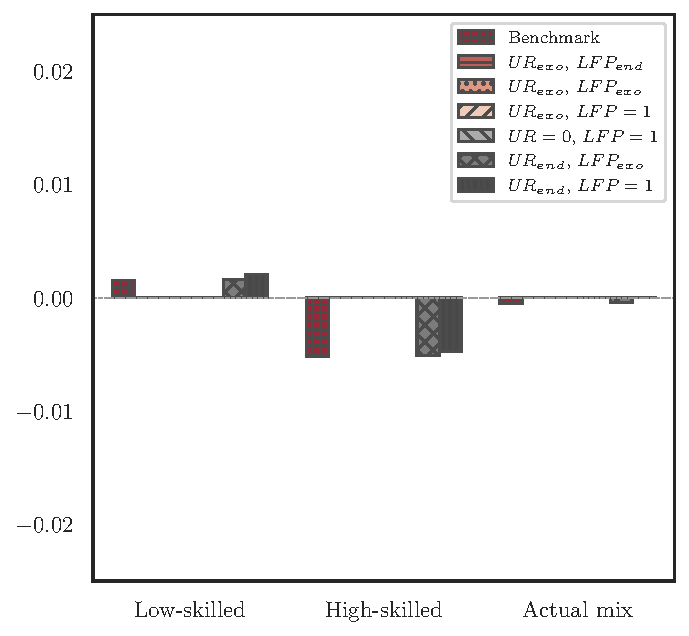
\includegraphics[width=\linewidth]{graphs/qURml.pdf}
% \end{subfigure}
% \hfill
% \begin{subfigure}{.3\linewidth}
%   \centering
%   \caption{${\frac{U_{mh}^{**}}{Q_{mh}^{**}}}/{\frac{U_{mh}^{*}}{Q_{mh}^{*}}}-1$} 
%   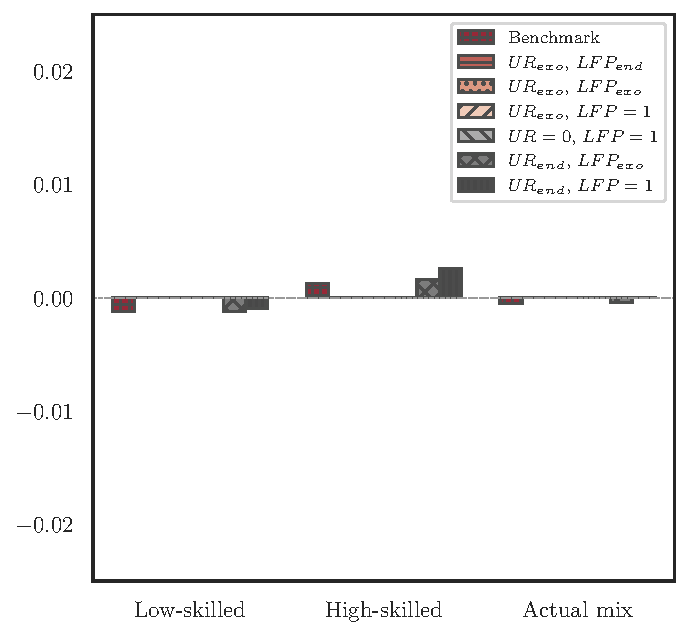
\includegraphics[width=\linewidth]{graphs/qURmh.pdf}
% \end{subfigure}
% \hfill
% \begin{subfigure}{.3\linewidth}
%   \centering
%   \caption{$
% {\frac{U_{ml}^{**}+U_{mh}^{**}}{Q_{ml}^{**}+Q_{mh}^{**}}}/{\frac{U_{ml}^{*}+U_{mh}^{*}}{Q_{ml}^{*}+Q_{mh}^{*}}}-1$} 
%   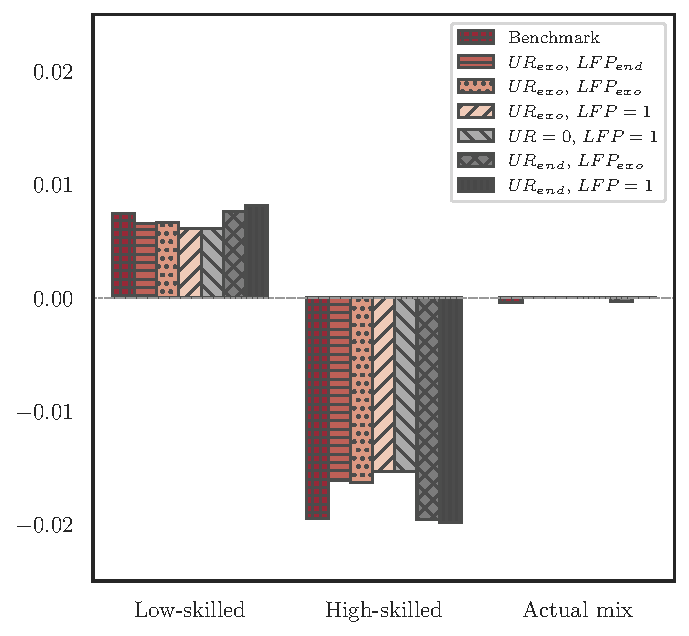
\includegraphics[width=\linewidth]{graphs/qURm.pdf}
% \end{subfigure}
% \\[0.5cm]
% \begin{subfigure}{.3\linewidth}
%   \centering
%   \caption{${\frac{U_{nl}^{**}}{Q_{nl}^{**}}}/{\frac{U_{nl}^{*}}{Q_{nl}^{*}}}-1$}
%   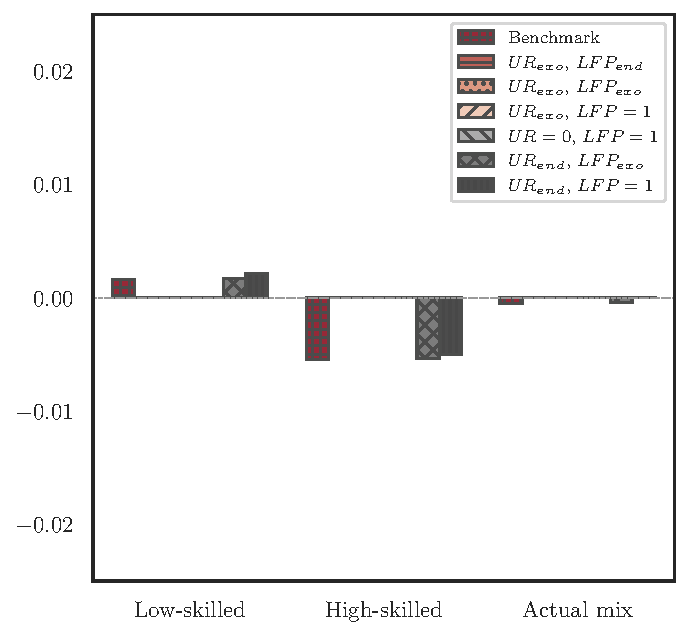
\includegraphics[width=\linewidth]{graphs/qnURnl.pdf}
% \end{subfigure}%
% \hfill
% \begin{subfigure}{.3\linewidth}
%   \centering
%   \caption{${\frac{U_{nh}^{**}}{Q_{nh}^{**}}}/{\frac{U_{nh}^{*}}{Q_{nh}^{*}}}-1$}
%   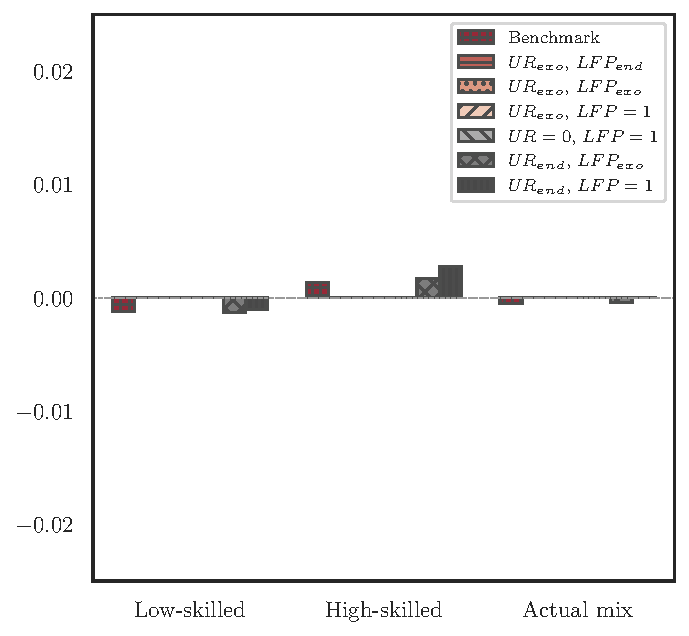
\includegraphics[width=\linewidth]{graphs/qnURnh.pdf}
% \end{subfigure}
% \hfill
% \begin{subfigure}{.3\linewidth}
%   \centering
%   \caption{${\frac{U_{nl}^{**}+U_{nh}^{**}}{Q_{nl}^{**}+Q_{nh}^{**}}}/{\frac{U_{nl}^{*}+U_{nh}^{*}}{Q_{nl}^{*}+Q_{nh}^{*}}}-1$}
%   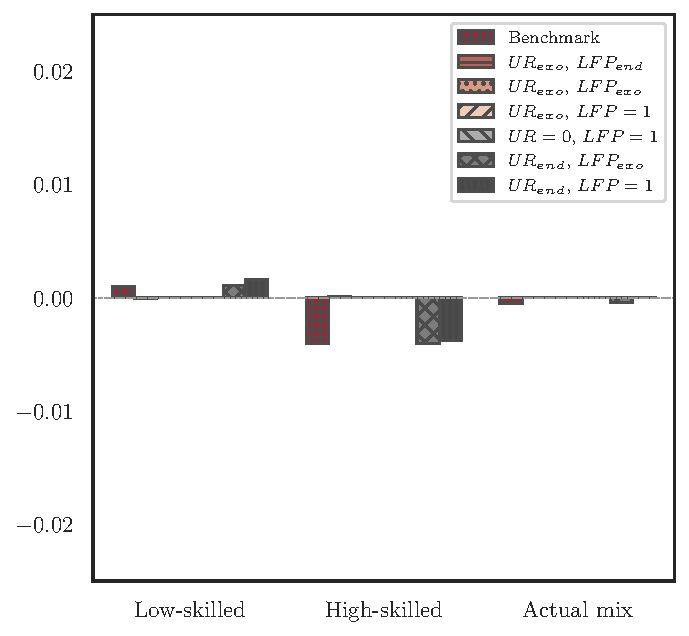
\includegraphics[width=\linewidth]{graphs/qnURn.pdf}
% \end{subfigure}
% \\[0.5cm]
% \end{figure}
% \end{landscape} \restoregeometry
% }

% \afterpage{
% \newgeometry{left=1cm,right=1cm,top=2cm,bottom=2cm,nohead}
% \begin{landscape}%
% \begin{center}
% \begin{figure}[htb!]
% \centering
% \caption{Average welfare effect of immigration (1\% of the total labor force) -- Sensitivity to $\eta$}
% \label{fig:welfare_sensitivity_eta}
% \begin{subfigure}{.45\linewidth}
%   \centering
%   \caption{Unweighted mean effect}
%   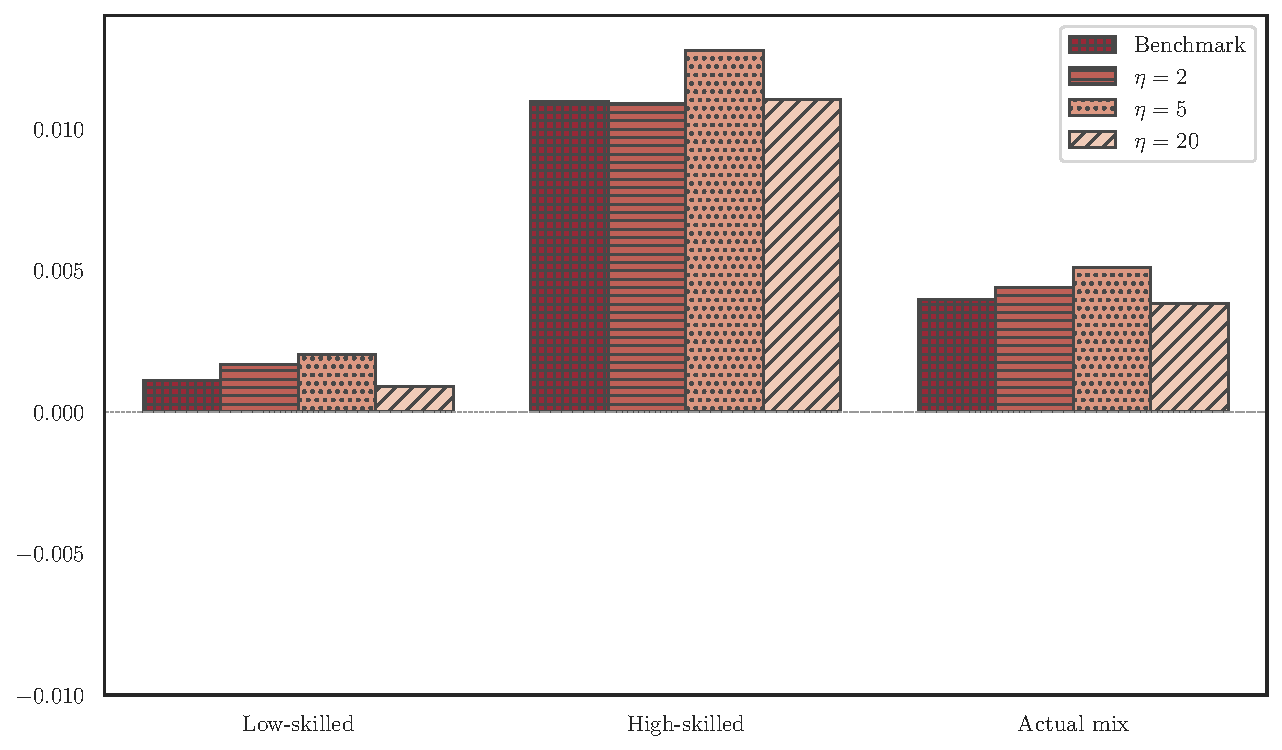
\includegraphics[width=\linewidth]{graphs/sens_eta_Welf.pdf}
% \end{subfigure}%
% \hfill
% \begin{subfigure}{.45\linewidth}
%   \centering
%     \caption{Effect by country: low-skilled immigration}
%   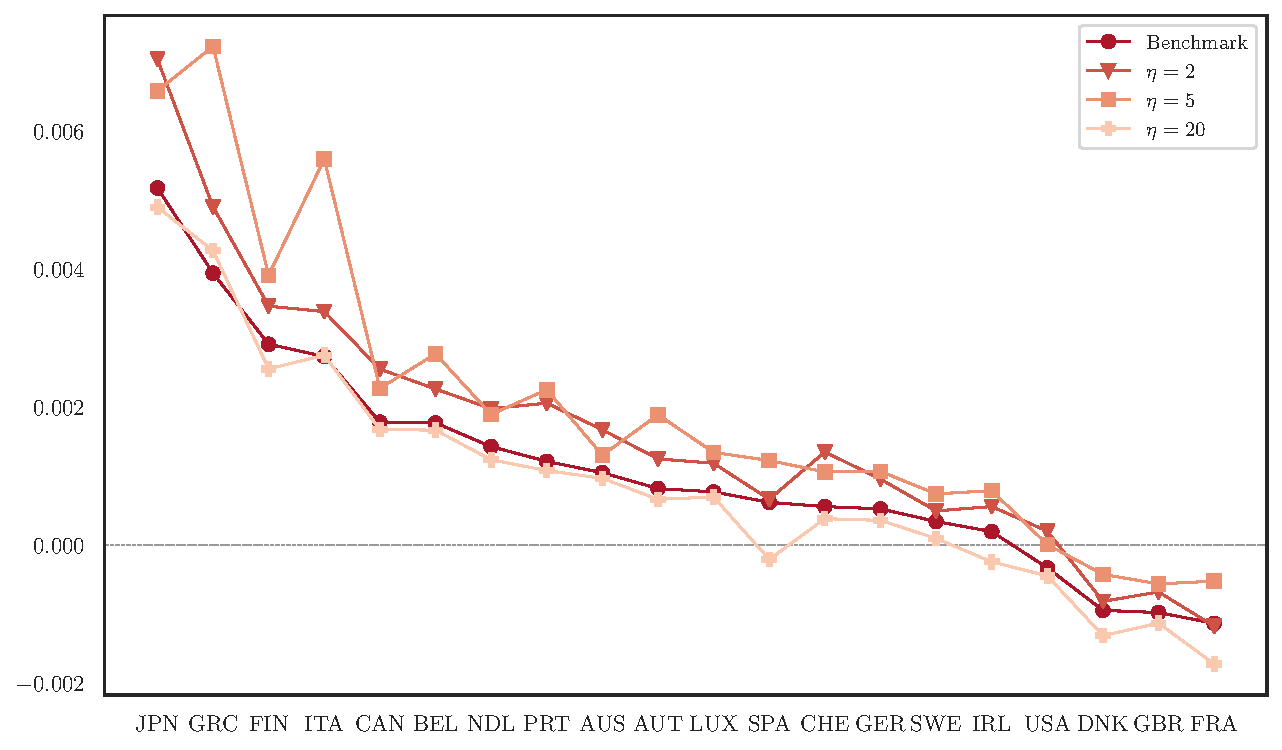
\includegraphics[width=\linewidth]{graphs/sens_eta_Welf_LS.pdf}
% \end{subfigure}
% \\[0.5cm]
% \begin{subfigure}{.45\linewidth}
%   \centering
%       \caption{Effect by country: high-skilled immigration}
%   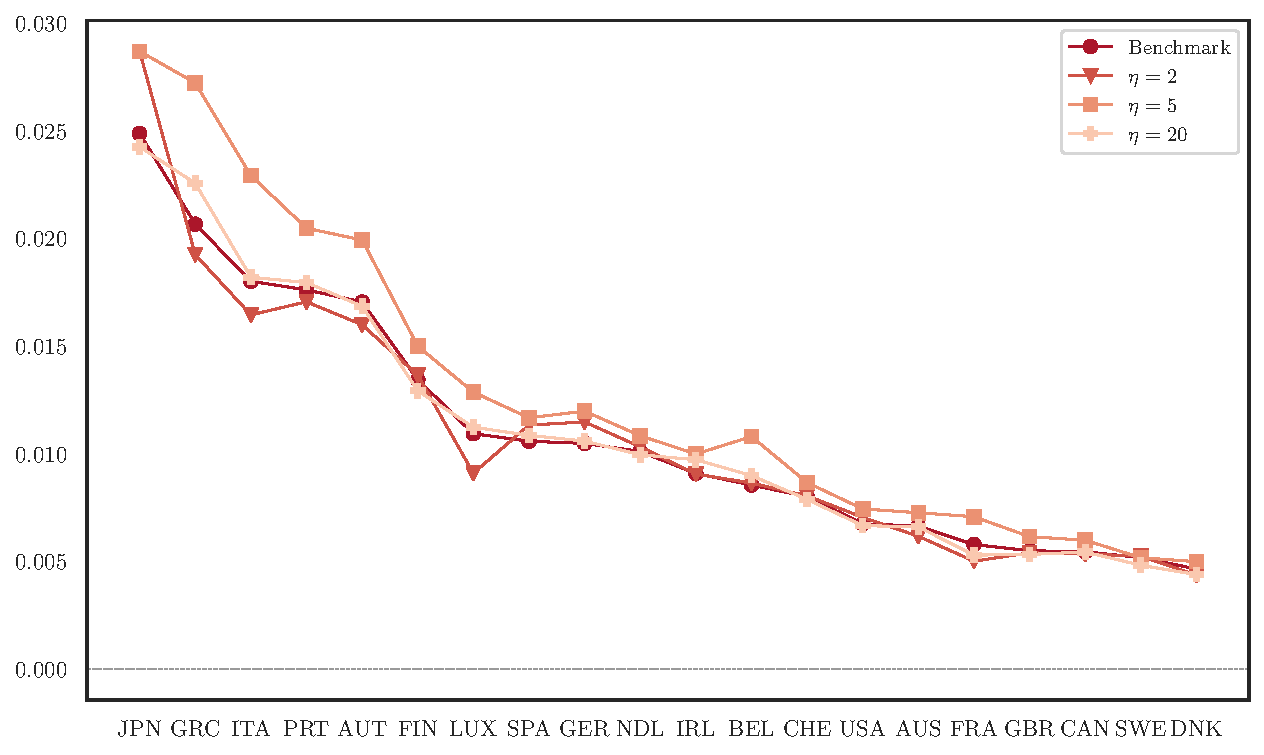
\includegraphics[width=\linewidth]{graphs/sens_eta_Welf_HS.pdf}
% \end{subfigure}%
% \hfill
% \begin{subfigure}{.45\linewidth}
%   \centering
%         \caption{Effect by country: actual education mix}
%   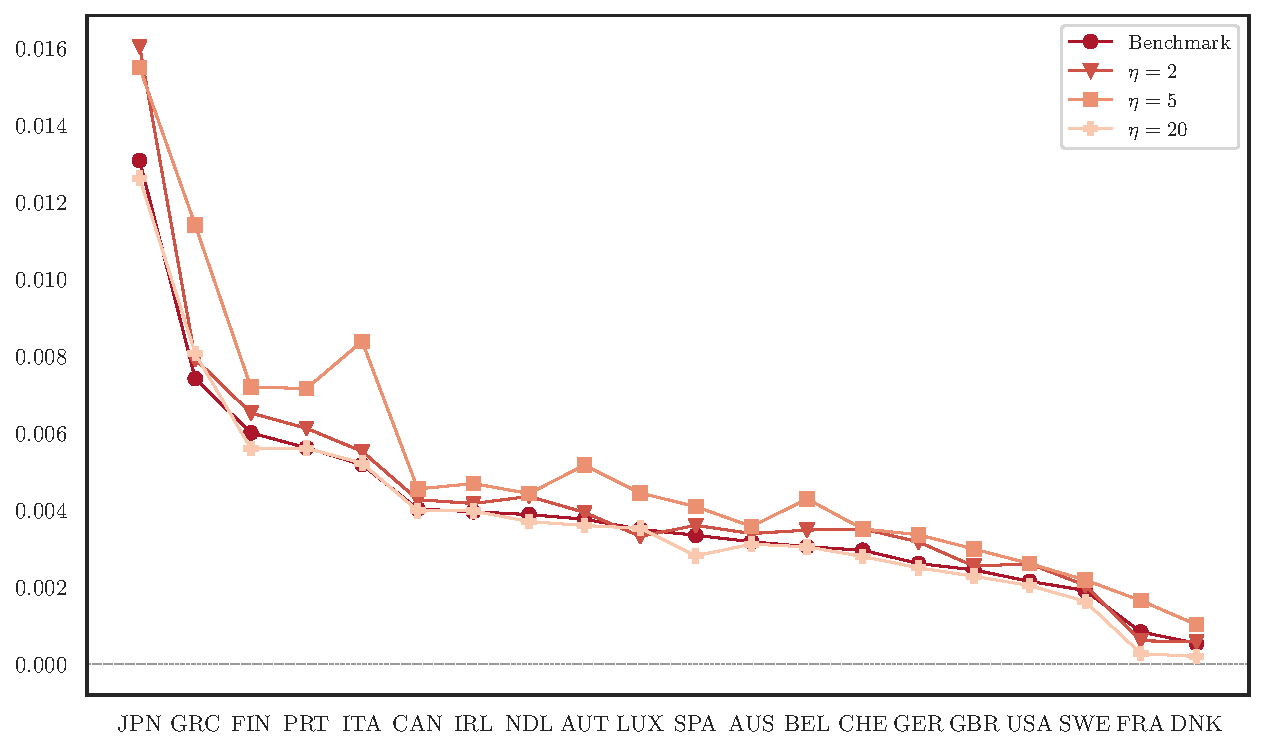
\includegraphics[width=\linewidth]{graphs/sens_eta_Welf_LS+HS.pdf}
% \end{subfigure}
% \\[0.5cm]
% {\footnotesize \textbf{Notes:} Figure~\ref{fig:welfare_sensitivity_eta} shows the results for 20 selected countries:\\ the 15 members states of the European Union (EU15), the US, Canada,
% Australia, Switzerland and Japan.}
% \end{figure}
% \end{center}
% \end{landscape}
% \restoregeometry 
% }

\section{Appendix}
\label{Appendix B}

The six transmission channels used to calculate Eq. (\ref{Eq:DecompPrivateCons2}) are weighted sums of skill-specific effects, which are given by:

\begin{eqnarray*}
\left. \frac{d\overline{\mathcal{U}}_{n}^{y}}{\overline{\mathcal{U}}_{n}^{y}}\right \vert_{partic} &=&\frac{\eta}{1+\eta} \left[
\frac{N_{n,h}^{y}\left( C_{n,h}^{y}-\frac{T_{n,h}^{y}}{(1-v)P}\right) }{\left(
N_{n,h}^{y}+N_{n,l}^{y}\right) \overline{\mathcal{U}}_{n}^{y}}\cdot \frac{d(1-\ell_{n,h}^{y})}{(1-\ell _{n,h}^{y})}+\frac{N_{n,l}^{y}\left(
C_{n,l}^{y}-\frac{T_{n,l}^{y}}{(1-v)P}\right) }{\left( N_{n,h}^{y}+N_{n,l}^{y}\right) 
\overline{\mathcal{U}}_{n}^{y}}\cdot \frac{d(1-\ell _{n,l}^{y})}{(1-\ell _{n,l}^{y})} \right] \\
\left. \frac{d\overline{\mathcal{U}}_{n}^{y}}{\overline{\mathcal{U}}_{n}^{y}}\right \vert_{wage}
&=&\frac{\eta}{1+\eta} \left[
\frac{N_{n,h}^{y}\left( C_{n,h}^{y}-\frac{T_{n,h}^{y}}{(1-v)P}\right) }{\left(
N_{n,h}^{y}+N_{n,l}^{y}\right) \overline{\mathcal{U}}_{n}^{y}}\cdot \frac{dw_{n,h}}{%
w_{n,h}}+\frac{N_{n,l}^{y}\left( C_{n,l}^{y}-\frac{T_{n,l}^{y}}{(1-v)P}\right) }{\left(
N_{n,h}^{y}+N_{n,l}^{y}\right) \overline{\mathcal{U}}_{n}^{y}}\cdot \frac{dw_{n,l}}{%
w_{n,l}} \right] \\
\left. \frac{d\overline{\mathcal{U}}_{n}^{y}}{\overline{\mathcal{U}}_{n}^{y}}\right \vert_{empl}
&=& \frac{\eta}{1+\eta} \left[
\frac{N_{n,h}^{y}\left( C_{n,h}^{y}-\frac{T_{n,h}^{y}}{(1-v)P}\right) }{\left(
N_{n,h}^{y}+N_{n,l}^{y}\right) \overline{\mathcal{U}}_{n}^{y}}\cdot \frac{d(1-u_{n,h})%
}{(1-u_{n,h})}+\frac{N_{n,l}^{y}\left( C_{n,l}^{y}-\frac{T_{n,l}^{y}}{(1-v)P}\right) }{%
\left( N_{n,h}^{y}+N_{n,l}^{y}\right) \overline{\mathcal{U}}_{n}^{y}}\cdot \frac{%
d(1-u_{n,l})}{(1-u_{n,l})} \right] \\
\left. \frac{d\overline{\mathcal{U}}_{n}^{y}}{\overline{\mathcal{U}}_{n}^{y}}\right \vert_{fiscal} &=&\frac{\eta}{1+\eta} \left[
\frac{N_{n,h}^{y}\left( C_{n,h}^{y}-\frac{T_{n,h}^{y}}{(1-v)P}\right) }{\left(
N_{n,h}^{y}+N_{n,l}^{y}\right) \overline{\mathcal{U}}_{n}^{y}}\cdot \frac{d(1-\tau )}{%
(1-\tau )}+\frac{N_{n,l}^{y}\left( C_{n,l}^{y}-\frac{T_{n,l}^{y}}{(1-v)P}\right) }{\left(
N_{n,h}^{y}+N_{n,l}^{y}\right) \overline{\mathcal{U}}_{n}^{y}}\cdot \frac{d(1-\tau )}{%
(1-\tau )} \right] \\
\left. \frac{d\overline{\mathcal{U}}_{n}^{y}}{\overline{\mathcal{U}}_{n}^{y}}\right \vert_{resid} &=&\frac{\eta}{1+\eta} \left[
\frac{N_{n,h}^{y}\left( C_{n,h}^{y}-\frac{T_{n,h}^{y}}{(1-v)P}\right) }{\left(
N_{n,h}^{y}+N_{n,l}^{y}\right) \overline{\mathcal{U}}_{n}^{y}}\cdot \frac{d\Gamma
_{n,h}^{y}}{\Gamma _{n,h}^{y}}+\frac{N_{n,l}^{y}\left(
C_{n,l}^{y}-\frac{T_{n,l}^{y}}{(1-v)P}\right) }{\left( N_{n,h}^{y}+N_{n,l}^{y}\right) 
\overline{\mathcal{U}}_{n}^{y}}\cdot \frac{d\Gamma _{n,l}^{y}}{\Gamma _{n,l}^{y}} \right] \\
\left. \frac{d\overline{\mathcal{U}}_{n}^{y}}{\overline{\mathcal{U}}_{n}^{y}}\right \vert_{price} &=&
-\frac{dP}{P}.
\end{eqnarray*}

Similarly, Eq. (\ref{Eq:DecompIneq}) is obtained by the sum of the following partial effects
\begin{eqnarray*}
\left. \frac{dI_{n}^{y}}{I_{n}^{y}}\right \vert _{partic} &=& \frac{\eta}{1+\eta} \left[
\frac{C_{n,h}^{y}-\frac{T_{n,h}^{y}}{(1-v)P}}{\mathcal{U}_{n,h}^{y}}\cdot \frac{d(1-\ell _{n,h}^{y})}{(1-\ell _{n,h}^{y})}-\frac{C_{n,l}^{y}-\frac{T_{n,l}^{y}}{(1-v)P}}{\mathcal{U}_{n,l}^{y}}\cdot \frac{d(1-\ell _{n,l}^{y})}{(1-\ell _{n,l}^{y})} \right] \\
\left. \frac{dI_{n}^{y}}{I_{n}^{y}}\right \vert _{wage} &=& \frac{\eta}{1+\eta} \left[
\frac{C_{n,h}^{y}-\frac{T_{n,h}^{y}}{(1-v)P}}{\mathcal{U}_{n,h}^{y}}\cdot \frac{dw_{n,h}}{w_{n,h}}-\frac{C_{n,l}^{y} -\frac{T_{n,l}^{y}}{(1-v)P}}{\mathcal{U}_{n,l}^{y}}\cdot \frac{dw_{n,l}}{w_{n,l}} \right] \\
\left. \frac{dI_{n}^{y}}{I_{n}^{y}}\right \vert _{empl} &=& \frac{\eta}{1+\eta} \left[
\frac{C_{n,h}^{y}-\frac{T_{n,h}^{y}}{(1-v)P}}{\mathcal{U}_{n,h}^{y}}\cdot \frac{d(1-u_{n,h})}{(1-u_{n,h})} -\frac{C_{n,l}^{y}-\frac{T_{n,l}^{y}}{(1-v)P}}{\mathcal{U}_{n,l}^{y}}\cdot \frac{d(1-u_{n,l})}{%
(1-u_{n,l})} \right] \\
\left. \frac{dI_{n}^{y}}{I_{n}^{y}}\right \vert _{fiscal} &=& \frac{\eta}{1+\eta} \left[
\frac{C_{n,h}^{y}-\frac{T_{n,h}^{y}}{(1-v)P}}{\mathcal{U}_{n,h}^{y}}\cdot \frac{d(1-\tau )}{(1-\tau )}
- \frac{C_{n,l}^{y}-\frac{T_{n,l}^{y}}{(1-v)P}^{y}}{\mathcal{U}_{n,l}^{y}}\cdot \frac{d(1-\tau )}{(1-\tau )} \right] \\
\left. \frac{dI_{n}^{y}}{I_{n}^{y}}\right \vert _{resid} &=& \frac{\eta}{1+\eta} \left[
\frac{C_{n,h}^{y}-\frac{T_{n,h}^{y}}{(1-v)P}}{\mathcal{U}_{n,h}^{y}}\cdot \frac{d\Gamma_{n,h}^{y}}{\Gamma_{n,h}^{y}}
-\frac{C_{n,l}^{y}-\frac{T_{n,l}^{y}}{(1-v)P}}{\mathcal{U}_{n,l}^{y}}\cdot \frac{d\Gamma_{n,l}^{y}}{\Gamma _{n,l}^{y}} \right] \\
\left. \frac{dI_{n}^{y}}{I_{n}^{y}}\right \vert _{price} &=& 0.
\end{eqnarray*}

\begin{comment}
\clearpage

\newgeometry{,left=1cm,right=1cm,top=2cm,bottom=2cm,nohead}
\begin{landscape}
\vspace*{\fill}
\begin{center}
\renewcommand{\arraystretch}{0.55}
\begin{figure}[htb!]
\caption{Average utility effect of immigration (1\% of the total labor
force) -- Sensitivity to labor market modeling}
\label{fig:DOO_utility_effects}
\centering
\begin{subfigure}{.45\linewidth}
\caption{Unweighted mean effect} \label{fig:DOO_utility_effects_a}
  \centering
  \includegraphics[width=\linewidth]{\DOOgraphPath Utility.pdf}
\end{subfigure}
\hfill
\begin{subfigure}{.45\linewidth}
  \centering
  \caption{Effect by country: low-skilled immigration} \label{fig:DOO_utility_effects_b}
  \includegraphics[width=\linewidth]{\DOOgraphPath Utility_LS.pdf}
\end{subfigure}
\\[0.5cm]
\begin{subfigure}{.45\linewidth}
  \centering
  \caption{Effect by country: high-skilled immigration} \label{fig:DOO_utility_effects_c}
  \includegraphics[width=\linewidth]{\DOOgraphPath Utility_HS.pdf}
\end{subfigure}%
\hfill
\begin{subfigure}{.45\linewidth}
  \centering
  \caption{Effect by country: actual education mix} \label{fig:DOO_utility_effects_d}
  \includegraphics[width=\linewidth]{\DOOgraphPath Utility_LS+HS.pdf}
\end{subfigure}
\\[0.5cm]
{\footnotesize \textbf{Notes:} Figure~\ref{fig:DOO_utility_effects} shows the results for 20 selected countries: the 15 members states of the European Union (EU15), the US, Canada,
Australia, Switzerland and Japan.}
\end{figure}
\end{center}
\vspace*{\fill}
\end{landscape}
\restoregeometry

\clearpage

\newgeometry{left=1cm,right=1cm,top=2cm,bottom=2cm,nohead}
\begin{landscape}
\begin{center}
\renewcommand{\arraystretch}{0.55}
\begin{figure}[htb!]
\centering
\caption{Decomposition of the average welfare effect of immigration (1\% of the total labor
force) -- Sensitivity to labor market modeling}
\label{fig:DOO_decomp}
\begin{subfigure}{.3\linewidth}
\caption{Wage effect} \label{fig:DOO_decomp_mean_W}
  \centering
  \includegraphics[width=\linewidth]{\DOOgraphPath qWn.pdf}
\end{subfigure}
\hfill
\begin{subfigure}{.3\linewidth}
  \centering
\caption{Employment effect} \label{fig:DOO_decomp_mean_UR}
  \includegraphics[width=\linewidth]{\DOOgraphPath qURn.pdf}
\end{subfigure}
\hfill
\begin{subfigure}{.3\linewidth}
  \centering
\caption{Labor force participation effect} \label{fig:DOO_decomp_mean_ln}
  \includegraphics[width=\linewidth]{\DOOgraphPath qln.pdf}
\end{subfigure}
\\[0.5cm]
\begin{subfigure}{.3\linewidth}
  \centering
\caption{Fiscal effect} \label{fig:DOO_decomp_mean_tau}
  \includegraphics[width=\linewidth]{\DOOgraphPath qTau.pdf}
\end{subfigure}%
\hfill
\begin{subfigure}{.3\linewidth}
  \centering
\caption{Price effect} \label{fig:DOO_decomp_mean_P}
  \includegraphics[width=\linewidth]{\DOOgraphPath qP.pdf}
\end{subfigure}
\hfill
\begin{subfigure}{.3\linewidth}
  \centering
\caption{Residual} \label{fig:DOO_decomp_mean_Resn}
  \includegraphics[width=\linewidth]{\DOOgraphPath qResn.pdf}
\end{subfigure}
\\[0.5cm]
{\footnotesize \textbf{Notes:} Figure~\ref{fig:DOO_decomp} shows the results for 20 selected countries:
the 15 members states of the European Union (EU15), the US, Canada,
Australia, Switzerland and Japan.}
\end{figure}
\end{center}
\end{landscape}
\restoregeometry

\clearpage

\newgeometry{,left=1cm,right=1cm,top=2cm,bottom=2cm,nohead}
\begin{landscape} 
\vspace*{\fill}
\begin{center}
\renewcommand{\arraystretch}{0.55}
\begin{figure}[htb!]
\centering
\caption{Inequality effect of immigration (1\% of the total labor force) -- Sensitivity to labor market modelling}
\label{fig:DOO_utility_inequality_effects}
\begin{subfigure}{.45\linewidth}
  \centering
  \caption{Unweighted mean effect} \label{fig:DOO_utility_inequality_effects_a}
  \includegraphics[width=\linewidth]{\DOOgraphPath UtilityIneq.pdf}
\end{subfigure}
\hfill
\begin{subfigure}{.45\linewidth}
  \centering
    \caption{Effect by country: low-skilled immigration} \label{fig:DOO_utility_inequality_effects_b}
  \includegraphics[width=\linewidth]{\DOOgraphPath UtilityIneq_LS.pdf}
\end{subfigure}
\\[0.5cm]
\begin{subfigure}{.45\linewidth}
  \centering
     \caption{Effect by country: high-skilled immigration} \label{fig:DOO_utility_inequality_effects_c}
  \includegraphics[width=\linewidth]{\DOOgraphPath UtilityIneq_HS.pdf}
\end{subfigure}
\hfill
\begin{subfigure}{.45\linewidth}
  \centering
    \caption{Effect by country: actual education mix} \label{fig:DOO_utility_inequality_effects_d}
  \includegraphics[width=\linewidth]{\DOOgraphPath UtilityIneq_LS+HS.pdf}
\end{subfigure}
\\[0.5cm]
{\footnotesize \textbf{Notes:} Figure~\ref{fig:DOO_utility_inequality_effects} shows the results for 20 selected countries: the 15 members states of the European Union (EU15), the US, Canada, Australia, Switzerland and Japan. }
\end{figure}
\end{center}
\vspace*{\fill}
\end{landscape}
\restoregeometry

\clearpage

\newgeometry{left=1cm,right=1cm,top=2cm,bottom=2cm,nohead}
\begin{landscape}
\begin{center}
\renewcommand{\arraystretch}{0.55}
\begin{figure}[htb!]
\centering
\caption{Decomposition of inequality effect of immigration (1\% of the total labor
force) -- Sensitivity to labor market modeling}
\label{fig:DOO_decomp_INC}
\begin{subfigure}{.3\linewidth}
\caption{Wage effect} \label{fig:DOO_decomp_mean_WINC}
  \centering
  \includegraphics[width=\linewidth]{\DOOgraphPath qWnINC.pdf}
\end{subfigure}
\hfill
\begin{subfigure}{.3\linewidth}
  \centering
  \caption{Employment effect} \label{fig:DOO_decomp_mean_URINC}
  \includegraphics[width=\linewidth]{\DOOgraphPath qURnINC.pdf}
\end{subfigure}
\hfill
\begin{subfigure}{.3\linewidth}
  \centering
  \caption{Labor force participation effect} \label{fig:DOO_decomp_mean_lnINC}
  \includegraphics[width=\linewidth]{\DOOgraphPath qlnINC.pdf}
\end{subfigure}
\\[0.5cm]
\begin{subfigure}{.3\linewidth}
  \centering
  \caption{Fiscal effect} \label{fig:DOO_decomp_mean_tauINC}
  \includegraphics[width=\linewidth]{\DOOgraphPath qTauINC.pdf}
\end{subfigure}%
\hfill
\begin{subfigure}{.3\linewidth}
  \centering
  \caption{Price effect} \label{fig:DOO_decomp_mean_PINC}
  \includegraphics[width=\linewidth]{\DOOgraphPath qPINC.pdf}
\end{subfigure}
\hfill
\begin{subfigure}{.3\linewidth}
  \centering
  \caption{Residual} \label{fig:DOO_decomp_mean_ResnINC}
  \includegraphics[width=\linewidth]{\DOOgraphPath qResnINC.pdf}
\end{subfigure}
\\[0.5cm]
{\footnotesize \textbf{Notes:} Figure~\ref{fig:DOO_decomp_INC} shows the results for 20 selected countries:
the 15 members states of the European Union (EU15), the US, Canada,
Australia, Switzerland and Japan.}
\end{figure}
\end{center}
\end{landscape}
\restoregeometry
\end{comment}
\end{document}
